% Options for packages loaded elsewhere
\PassOptionsToPackage{unicode}{hyperref}
\PassOptionsToPackage{hyphens}{url}
\documentclass[
]{article}
\usepackage{xcolor}
\usepackage[margin=1in]{geometry}
\usepackage{amsmath,amssymb}
\setcounter{secnumdepth}{-\maxdimen} % remove section numbering
\usepackage{iftex}
\ifPDFTeX
  \usepackage[T1]{fontenc}
  \usepackage[utf8]{inputenc}
  \usepackage{textcomp} % provide euro and other symbols
\else % if luatex or xetex
  \usepackage{unicode-math} % this also loads fontspec
  \defaultfontfeatures{Scale=MatchLowercase}
  \defaultfontfeatures[\rmfamily]{Ligatures=TeX,Scale=1}
\fi
\usepackage{lmodern}
\ifPDFTeX\else
  % xetex/luatex font selection
\fi
% Use upquote if available, for straight quotes in verbatim environments
\IfFileExists{upquote.sty}{\usepackage{upquote}}{}
\IfFileExists{microtype.sty}{% use microtype if available
  \usepackage[]{microtype}
  \UseMicrotypeSet[protrusion]{basicmath} % disable protrusion for tt fonts
}{}
\makeatletter
\@ifundefined{KOMAClassName}{% if non-KOMA class
  \IfFileExists{parskip.sty}{%
    \usepackage{parskip}
  }{% else
    \setlength{\parindent}{0pt}
    \setlength{\parskip}{6pt plus 2pt minus 1pt}}
}{% if KOMA class
  \KOMAoptions{parskip=half}}
\makeatother
\usepackage{longtable,booktabs,array}
\usepackage{caption}
\captionsetup[table]{skip=6pt}
\newcounter{none} % for unnumbered tables
\usepackage{calc} % for calculating minipage widths
% Correct order of tables after \paragraph or \subparagraph
\usepackage{etoolbox}
\makeatletter
\patchcmd\longtable{\par}{\if@noskipsec\mbox{}\fi\par}{}{}
\makeatother
% Allow footnotes in longtable head/foot
\IfFileExists{footnotehyper.sty}{\usepackage{footnotehyper}}{\usepackage{footnote}}
\makesavenoteenv{longtable}
\usepackage{graphicx}
\makeatletter
\newsavebox\pandoc@box
\newcommand*\pandocbounded[1]{% scales image to fit in text height/width
  \sbox\pandoc@box{#1}%
  \Gscale@div\@tempa{\textheight}{\dimexpr\ht\pandoc@box+\dp\pandoc@box\relax}%
  \Gscale@div\@tempb{\linewidth}{\wd\pandoc@box}%
  \ifdim\@tempb\p@<\@tempa\p@\let\@tempa\@tempb\fi% select the smaller of both
  \ifdim\@tempa\p@<\p@\scalebox{\@tempa}{\usebox\pandoc@box}%
  \else\usebox{\pandoc@box}%
  \fi%
}
% Set default figure placement to htbp
\def\fps@figure{htbp}
\makeatother
\setlength{\emergencystretch}{3em} % prevent overfull lines
\providecommand{\tightlist}{%
  \setlength{\itemsep}{0pt}\setlength{\parskip}{0pt}}
\usepackage{graphicx}
\graphicspath{{figures/}{./}}
\usepackage{bookmark}
\IfFileExists{xurl.sty}{\usepackage{xurl}}{} % add URL line breaks if available
\urlstyle{same}
% fallback for those not using the hyperref driver hyperxmp:
\makeatletter
\@ifundefined{xmpquote}{\newcommand{\xmpquote}[1]{#1}}{}
\makeatother
\hypersetup{
  hidelinks,
  pdfcreator={LaTeX via pandoc}}

\author{}
\date{\vspace{-2.5em}}

\begin{document}

\section{Tournaments not inducible by five
voters}\label{tournaments-not-inducible-by-five-voters}

\textbf{Leonid Chindelevitch\(^{1}\) and Ararat Harutyunyan\(^{2}\)}

\(^{1}\) MRC Centre for Global Infectious Disease Analysis, School of
Public Health, Imperial College London, London, United Kingdom. Email:
\texttt{lchindel@ic.ac.uk}. ORCID: 0000-0002-6619-6013.

\(^{2}\) University of Paris-Dauphine, PSL University, CNRS UMR7243,
LAMSADE, Paris, France. Email:
\texttt{ararat.harutyunyan@lamsade.dauphine.fr}.

Corresponding author: Leonid Chindelevitch (\texttt{lchindel@ic.ac.uk}).

\subsection{Abstract}\label{abstract}

How many voters must a committee have before its majority preferences
can take any form at all? A tournament is \(k\)-inducible if some \(k\)
linear orders produce it as their pairwise-majority relation, and for
odd \(k\) we write \(N(k)\) for the least number of alternatives at
which some tournament is not \(k\)-inducible. Only \(N(3) = 8\) is known
exactly. For five voters the best bounds were \(12 \le N(5) \le 38\),
and the smallest explicit tournament beyond five voters had \(43\)
vertices.

We improve both bounds to \(13 \le N(5) \le 22\). The upper bound comes
from two tournaments on \(22\) vertices, each a doubly regular
tournament on \(23\) vertices with one vertex deleted, that five voters
cannot produce; one of the two refutations is formally certified. On the
way we show that the Paley tournament on \(23\) vertices is not
\(5\)-inducible, a case a general-purpose SAT solver had left open after
six weeks, and that no doubly regular tournament on \(23\) vertices is.
The lower bound comes from an analysis of all tournaments on \(12\)
vertices. We also show that the Paley tournament on \(19\) vertices is
\(5\)-inducible, but not when every majority is carried by three voters
against two, and we determine which obstructions survive deleting a
vertex or reversing an arc. The method is a search that places one
alternative at a time, always the one with the fewest options left, and
exploits the symmetries of the tournament. Its negative results are
certified by machine-checkable proofs, and all results are reproducible
from a public repository.

\textbf{Keywords:} majority voting; tournaments; McGarvey's theorem;
Paley tournaments; constraint search; SAT

\begin{center}\rule{0.5\linewidth}{0.5pt}\end{center}

\subsection{1. Introduction}\label{introduction}

Majority rule imposes no structure at all on collective preference when
the electorate is unconstrained. For any pattern of pairwise majorities
one cares to specify, cycles and all, some profile of voters produces
exactly that pattern (McGarvey 1953); the Condorcet paradox is the
smallest instance of this freedom rather than an exception to it. What
makes the observation bite is that it needs \emph{many} voters, and the
question of how many is the question this paper is about.

Once the electorate is fixed, the freedom disappears. A panel of \(k\)
voters admits only finitely many profiles, so it can produce only
finitely many patterns of pairwise majority, and once the number of
alternatives is large enough most patterns are beyond it. A pattern that
some \(k\)-voter panel does produce we call \emph{\(k\)-inducible}. The
question is then one about small deliberative bodies: on an agenda of
\(n\) alternatives, is a committee of \(k\) members expressive enough to
realise every collective preference one could write down, or are there
patterns of majority preference that \(k\) members can never produce,
however they rank the alternatives?

For three voters the answer is known. Every pattern on at most seven
alternatives is realisable, and on eight alternatives one is not, by the
work of Shepardson and Tovey (2009) and of Eggermont, Hurkens and
Woeginger (2013). We write \(N(k)\) for the least number of alternatives
at which some pattern escapes \(k\) voters, so that \(N(3) = 8\). For
five voters -- the smallest committee size at which the question is
open, and a common size for panels, benches and selection committees --
the answer was known only to lie between \(12\) and \(38\), and no
explicit pattern on fewer than \(43\) alternatives was known to escape
five voters.

This paper narrows that to \(13 \le N(5) \le 22\), and both ends are
constructive. Five voters suffice on every agenda of at most twelve
alternatives: we verify this for all \(\approx 9.0 \times 10^{8}\)
patterns on eleven alternatives together with all of their
one-alternative extensions. And on twenty-two alternatives there are
patterns that five voters cannot produce: two tournaments, each obtained
by removing one alternative from a doubly regular tournament on
twenty-three. The first step on that way is the Paley tournament
\(P_{23}\) on twenty-three alternatives -- the instance a
general-purpose SAT solver failed to decide in six weeks of computation
in the work of Bachmeier et al.~(2019), which our search settles in
twenty-two hours on a laptop.

The pattern that first defeated five voters is worth describing in
words, because it is not a pathology. \(P_{23}\) is as balanced as a
collective preference on twenty-three alternatives can be: every
alternative defeats exactly eleven others, and every pair of
alternatives jointly defeats exactly the same number. It is the least
decisive pattern available, in the sense that no alternative and no pair
is distinguished from any other. That is precisely what a small panel
cannot manufacture. A committee of five produces its majorities by
accumulating agreement across five rankings, and the arithmetic of doing
so leaves traces -- some alternative better served than another, some
pair more often aligned. Perfect balance admits no such traces. The
obstruction to representation by a small electorate is therefore
balance, not irregularity, which is the opposite of what a reader
expecting hard instances to look messy would guess. Nor is it symmetry:
\(P_{23}\) is also highly symmetric, but the other \(36\) doubly regular
tournaments on twenty-three alternatives are just as balanced, \(32\) of
them have no symmetry at all, and all of them escape five voters too
(Section 3.7).

Two further findings sharpen the picture, and both concern \emph{how} a
majority is carried rather than whether it exists. A five-member panel
can carry a pairwise majority by three votes to two, by four to one, or
unanimously, and it is natural to ask whether the bare three-to-two
margins suffice. They do not: \(P_{19}\) is realisable by five voters,
but every profile realising it must carry some majority by more than the
bare minimum (Section 3.4). And the failures are fragile in a precise
sense: reversing a single pairwise majority in \(P_{19}\) or in
\(P_{23}\) restores realisability (Sections 3.3 and 3.6). A pattern out
of reach of five voters is thus not out of reach by a comfortable margin
-- it sits one pairwise comparison away from being realisable.

We follow the notation of our companion paper (Chindelevitch and
Harutyunyan 2026) throughout, which we briefly restate here. Let \(T\)
be a \emph{tournament} on the vertex set \(V\), \(|V| = n\): a digraph
in which every unordered pair \(\{i,j\}\) carries exactly one of the
arcs \(i \to j\) or \(j \to i\). A \emph{\(k\)-profile} consists of
\(k\) linear orders \(\pi_1, \dots, \pi_k\) on \(V\). The \emph{majority
tournament} of such a profile puts an arc from \(i\) to \(j\) whenever
\(|\{ v : i \prec_{\pi_v} j \}| > k/2\). For odd \(k\) this is
well-defined on every pair, and the result is a tournament. We say \(T\)
is \emph{\(k\)-inducible} if some \(k\)-profile has \(T\) as its
majority tournament, and we call such a profile a \emph{witness} for
\(T\). The \emph{converse} of \(T\) is the tournament obtained from
\(T\) by reversing the direction of every arc.

We call the number of voters who rank \(i\) above \(j\) the
\emph{support} of the arc \(e: i \to j\), and denote it \(c(e)\). If
\(c(e) > k/2\), the \emph{margin} of \(e\) is \(2c(e) - k\). In a
witness every arc's support exceeds \(k/2\), so for \(k = 5\) it is
\(3\), \(4\) or \(5\). A witness has \emph{margin at most \(M\)} if
every arc has margin at most \(M\). For \(k = 5\) the possible margins
are \(1\), which we call \emph{unit margin}, \(3\) (every support in
\(\{3,4\}\)), and \(5\) (no restriction, i.e.~plain majority). A
unit-margin witness is in particular a majority witness. In
Chindelevitch and Harutyunyan (2026) we conjectured that the
margin-based hierarchy is strict, which for \(k = 5\) asserts two
separate things: that some tournament is \(5\)-inducible with margin at
most \(3\) but not with unit margin, and that some tournament is
\(5\)-inducible but not with margin at most \(3\). We settle the first
here since \(P_{19}\) is such a tournament (Section 3.4), while the
second remains open (Section 4.2).

One further quantity recurs below. Informally, the \emph{predictability}
\(\alpha^{*}(T)\) is the largest fraction \(\alpha > 1/2\) for which
there is some profile, on any number \(t\) of voters, such that every
arc of \(T\) is supported by at least \(\alpha t\) of them; it is the
value of a linear program over the linear orders of \(V\). Since every
arc of a \(k\)-voter witness is supported by more than \(k/2\) of the
voters, \(k\)-inducibility forces \(\alpha^{*}(T) \ge (k+1)/2k\), which
is \(\tfrac{2}{3}\) at \(k = 3\) and \(\tfrac{3}{5}\) at \(k = 5\). The
implication is only one-directional: \(\alpha^{*}\) can meet the
threshold and the tournament still fail to be inducible. Shepardson and
Tovey (2009) introduced the notion; see Section 1.4 in Chindelevitch and
Harutyunyan (2026) for the computations and the counterexamples at both
\(k = 3\) and \(k = 5\).

Counting arguments show that almost all tournaments fail to be
\(k\)-inducible for any fixed \(k\), yet the \emph{explicit} examples
they yield are astronomically large. This paper closes much of the gap
for \(k = 5\). Let \(N(k)\) be the least order of a tournament that is
not \(k\)-inducible. The answer is only known exactly for \(k = 3\). For
\(k = 5\) the state of the art before this work was
\[12 \le N(5) \le 38,\] both ends of which are due to our companion
paper (Chindelevitch and Harutyunyan 2026): the lower bound came from an
exhaustive census of all \(\approx 9.0 \times 10^{8}\) tournaments on
\(11\) vertices, all of which admit a unit-margin five-voter profile,
improving on the bound \(N(5) \ge 11\) of Bachmeier et al.~(2019).

The upper bounds in the literature are of two different kinds and they
are not always comparable. Some are non-constructive, and obtained by
counting: one compares the number of tournaments of a given order with
the number that \(k\) linear orders can produce, and when the first
exceeds the second, some tournament of that order must be missed.
Bachmeier et al.~(2019) argued this way to reach \(41\), and
Chindelevitch and Harutyunyan (2026) sharpened the comparison by
restricting it to regular and near-regular tournaments, reaching \(38\).
Other bounds are constructive, and exhibit an explicit tournament. The
record for \(k = 5\) was \(P_{z}\) on \(z = 603{,}979{,}799\) vertices
(Bachmeier et al.~2019), from a dominating-set theorem of Alon et
al.~(2006) together with a construction of Graham and Spencer (1971),
which we improved to \(P_{43}\) (Chindelevitch and Harutyunyan 2026),
the first example of moderate order. Our bespoke algorithmic decision
procedure shows that \(P_{23}\) is not \(5\)-inducible, which improves
both the best non-constructive (counting) as well as the best
constructive (explicit) upper bounds to \(N(5) \le 23\), and then that
two tournaments on \(22\) vertices are not \(5\)-inducible either, so
that \(N(5) \le 22\).

\subsubsection{1.1 Special properties of Paley
tournaments}\label{special-properties-of-paley-tournaments}

The Paley tournament \(P_q\), for a prime \(q \equiv 3 \pmod 4\), has
vertex set \(\mathbb{F}_q\) and an arc from \(i\) to \(j\) whenever
\(j - i\) is a nonzero square, or \emph{quadratic residue}; we write
\(\mathrm{QR}\) for the set of these, so that \(i \to j\) exactly when
\(j - i \in
\mathrm{QR}\). As everywhere in this paper, vertices are numbered from
\(1\), vertex \(i + 1\) being the field element \(i\). It is
\emph{doubly regular}: every vertex has out-degree \((q-1)/2\) and every
ordered pair of vertices has exactly \((q-3)/4\) common out-neighbours.
Its automorphism group, written \(\mathrm{Aut}(P_q)\) and formally
defined in Section 2, has order \(q(q-1)/2\). This makes \(P_q\)
\emph{arc-transitive}, meaning that for every pair of arcs \(e, e'\) of
\(P_q\) there is an automorphism of \(P_q\) that takes \(e\) into
\(e'\). It is also \emph{self-converse}, meaning that it is isomorphic
to its own converse; the relevant mapping is simply multiplication by
\(-1\), which is easily checked to not be an automorphism when
\(q \equiv 3 \pmod 4\).

\subsubsection{1.2 Why Paley(23) is hard to classify and Paley(43) was
easy}\label{why-paley23-is-hard-to-classify-and-paley43-was-easy}

Paley tournaments are natural candidates for non-inducibility because
they are far from being transitive, and because their symmetry makes an
otherwise hopeless search merely very hard. Bachmeier et al.~(2019) call
them \emph{quadratic residue tournaments} and write \(Q_q\); their
orientation is the converse of ours. Since reversing every voter's order
reverses every arc of the majority tournament and changes no support, a
tournament and its converse have the same \emph{majority dimension}, the
least \(k\) for which a tournament is \(k\)-inducible, and are inducible
at exactly the same margins. We use the name Paley and the notation
\(P_q\) throughout.

The SAT study of Bachmeier et al.~(2019) establishes
\[\dim(Q_3) = \dim(Q_7) = 3, \qquad \dim(Q_{11}) = \dim(Q_{19}) = 5,\]
where \(\dim\) denotes majority dimension, and then stops exactly where
the problem becomes hard:

\begin{quote}
``Unfortunately, we were not able to check whether the majority
dimension of \(Q_{23}\) is equal to 5 or larger as the SAT solver did
not terminate within a total of six weeks.''
\end{quote}

By contrast, our previous proof that \(P_{43}\) is not \(5\)-inducible
(Chindelevitch and Harutyunyan 2026) never searched the profile space in
general. It rests on a quantity we call the \emph{slack},
\[\mathrm{slack}_5(T) = 5\,\mathrm{MAS}(T) - 3C, \qquad C = \binom{n}{2},\]
where \(\mathrm{MAS}\) is the maximum number of arcs of \(T\) that a
single linear order can agree with. Summing the majority condition over
all arcs bounds how far the five voters can \emph{collectively} fall
short of that maximum. A small slack restricts the voters to be close to
the best orders, and at \(q = 43\), where \(\mathrm{slack}_5 = 6\), that
restriction allowed us to fully enumerate about \(1.8\) million cases.

While the same argument is valid at every \(q\), the slack is \emph{not}
a monotone function of \(q\) (table from Chindelevitch and Harutyunyan
2026):

{\def\LTcaptype{none} % do not increment counter
\begin{longtable}[]{@{}lllllll@{}}
\toprule\noalign{}
\(q\) & 7 & 11 & 19 & 23 & 31 & 43 \\
\midrule\noalign{}
\endhead
\bottomrule\noalign{}
\endlastfoot
\(\mathrm{slack}_5\) & 7 & 10 & 22 & \textbf{46} & 30 & \textbf{6} \\
\end{longtable}
}

Since \(P_{43}\) attains a locally minimal slack, while \(P_{23}\)
attains a local maximum, the method of Chindelevitch and Harutyunyan
(2026) is unusable at \(q = 23\). For any \(q\),
\[\mathrm{slack}_5(P_q) \;=\; 5C\left(\alpha^{*}(P_q) - \tfrac{3}{5}\right),\]
where \(\alpha^{*}\) is the predictability; equality holds because
\(P_q\) is arc-transitive (Chindelevitch and Harutyunyan 2026). In
particular, the necessary condition \(\alpha^{*} \ge 3/5\) is far from
binding, so no argument resting on the predictability can certify
infeasibility.

\textbf{Predictability separates \(k = 5\) from \(k = 3\).} At \(k = 3\)
predictability decides exactly at \(N(3)\): the \(96\) non-3-inducible
tournaments on eight vertices have \(\alpha^{*} = \tfrac{13}{20}\),
which is \emph{below} \(\tfrac{2}{3}\), so the relaxation detects them,
while all other tournaments on eight vertices or fewer with at least one
cycle have \(\alpha^{*} = 2/3\) (Shepardson and Tovey 2009), and
\(N(3) = 8\) follows. At \(k = 5\) it does not: the table above has
\(\alpha^{*} > \tfrac{3}{5}\) at every \(q\), yet \(P_{23}\), \(P_{31}\)
and \(P_{43}\) are all non-inducible, with \(P_{23}\) being the farthest
\emph{above} the threshold among the three.

\subsubsection{1.3 Contributions}\label{contributions}

\begin{enumerate}
\def\labelenumi{\arabic{enumi}.}
\item
  \textbf{\(N(5) \le 22\)} (Section 3.2). Two non-isomorphic tournaments
  on \(22\) vertices, each a doubly regular tournament on \(23\)
  vertices with one vertex deleted, are not \(5\)-inducible, and both
  are vertex-critical. One of the two refutations is formally certified
  (Appendix B).
\item
  \textbf{\(P_{23}\) is not \(5\)-inducible} (Section 3.1). This settles
  the instance on which the SAT solver of Bachmeier et al.~(2019) did
  not terminate within a cumulative six weeks, and was the first step
  from \(38\) down to \(23\). We also decide \(P_{31}\), which does not
  improve the bound but demonstrates the method's reach: the larger
  tournament is settled in less time than \(P_{23}\).
\item
  \textbf{\(P_{19}\) is \(5\)-inducible, but not \(5\)-inducible with
  unit margin} (Section 3.4). This is an example suggesting that
  \(k = 5\) may qualitatively differ from \(k = 3\). For \(k = 3\), the
  first \(k\)-inducible tournaments that are non-\(k\)-inducible with
  unit margin appear after \(N(k)\), order 9 vs order 8 (Chindelevitch
  and Harutyunyan 2026). For \(k = 5\) they appear no later than order
  \(19\), so the order is reversed unless \(N(5) \le 19\), which the
  search of Appendix G argues against.
\item
  \textbf{\(P_{19}\) and \(P_{23}\) are arc-critical} (Sections 3.3 and
  3.6). Reversing an arc in \(P_{19}\) restores \(5\)-inducibility at
  unit margin, and reversing an arc in \(P_{23}\) restores unrestricted
  \(5\)-inducibility.
\item
  \textbf{\(P_{31}\) and \(P_{43}\) are not vertex-critical} (Section
  3.5). Deleting a vertex from \(P_{31}\) or \(P_{43}\) leaves a
  tournament that is still not \(5\)-inducible.
\item
  \textbf{Three formally certified negative results} (Appendix B).
  \(P_{19}\) is not \(5\)-inducible at unit margin, and \(P_{23}\) and
  \(\Delta_6 - 5\) are not \(5\)-inducible. The search is split into
  independent subproblems (\emph{cubes}); each is refuted by the SAT
  solver CaDiCaL, which emits its refutation as a machine-checkable
  \emph{LRAT} proof; and every one of those proofs is then rechecked by
  a separate program that shares no code with the solver.
\item
  \textbf{Every tournament on \(12\) vertices is \(5\)-inducible}
  (Appendix C). The analysis settles all \(2{,}048\) one-vertex
  extensions of each of the \(\approx 9.0 \times 10^{8}\) tournaments on
  \(11\) vertices, which is complete because every \(12\)-vertex
  tournament is such an extension of each of its twelve one-vertex
  deletions.
\end{enumerate}

\subsubsection{1.4 Related work}\label{related-work}

Two papers stand immediately behind this one, in different ways. Our
companion paper (Chindelevitch and Harutyunyan 2026) is the prior art
for the \emph{bound}: it produced the first explicit non-\(5\)-inducible
tournament of modest size, \(P_{43}\), and its two bounds are what we
measure against: \(N(5) \le 38\) by counting and \(N(5) \le 43\)
explicitly. Bachmeier et al.~(2019) is the prior art for the
\emph{problem and the method}: it brought SAT to bear on \(k\)-majority
digraphs, characterised the \(3\)-majority case building on Dushnik and
Miller (1941), and established hardness results for voting with a
constant number of voters.

The value of \(N(3)\) is settled. Shepardson and Tovey (2009) introduced
the predictability \(\alpha^{*}(T)\) defined above. A \(3\)-voter
profile is exactly a \(\tfrac{2}{3}\)-supermajority representation, so
\(\alpha^{*}(T) < \tfrac{2}{3}\) rules out \(3\)-inducibility; their
\(8\)-vertex tournament has \(\alpha^{*} = \tfrac{13}{20}\), which gives
\(N(3) \le 8\). They also prove that every tournament on at most \(7\)
vertices has \(\alpha^{*} \in \{\tfrac{2}{3}, 1\}\), and Eggermont,
Hurkens and Woeginger (2013) then show by direct computation using an
ILP formulation that every tournament on \(7\) vertices is
\(3\)-inducible, and every tournament on \(8\) or \(9\) vertices is
\(5\)-inducible, yielding \(N(3) = 8\) and \(N(5) \ge 10\).

Our certified computation (Appendix B.1) is standard. It splits the
problem into independent subproblems, using the \emph{cube-and-conquer}
paradigm (Heule et al.~2012): a SAT instance is split by fixing a few
variables at a time, giving many partial assignments called
\emph{cubes}, and each cube is handed to the solver as a problem of its
own. We adopt the standard of evidence set by the Boolean Pythagorean
triples proof (Heule et al.~2016; Cruz-Filipe et al.~2019), in which
every subproblem emits a machine-checkable refutation that an
independent checker validates. Our refutations are in the LRAT format
(Cruz-Filipe et al.~2017) (Appendix B.1), a format in which the solver
records each clause it derives so that an independent checker can replay
and confirm the entire derivation.

This paper grew out of our companion paper (Chindelevitch and
Harutyunyan 2026), whose constructive bound \(N(5) \le 43\) came from a
structural argument, and whose counting bound \(N(5) \le 38\) names no
explicit tournament. The question of what a genuine decision procedure
would reach at smaller orders led to the search of Appendix A.

The rest of this paper is organised as follows. Section 2 sets out the
notation, the symmetry reductions and the search in outline. Section 3
presents the results: \(P_{23}\) and \(P_{31}\) (Section 3.1), the two
\(22\)-vertex obstructions that give \(N(5) \le 22\) (Section 3.2),
vertex- and arc-criticality (Sections 3.3 to 3.6), and other structured
families (Section 3.7). Section 4 discusses where the method may
transfer and what remains open, and Section 5 describes the
reproducibility material. Appendix A describes the search engine and the
cost of every computation, Appendix B the formal certificates, Appendix
C the analysis of order \(12\), Appendix D the exact enumeration counts,
Appendix E the construction for locally transitive tournaments, Appendix
F criticality at \(21\) vertices, and Appendix G the search below \(22\)
vertices.

\begin{center}\rule{0.5\linewidth}{0.5pt}\end{center}

\subsection{2. Preliminaries}\label{preliminaries}

Throughout, \(T\) is a tournament on \(V = \{1, \dots, n\}\) and
\(k = 5\) unless stated otherwise. We write \(N^{+}(v)\) and
\(N^{-}(v)\) for the out- and in-neighbourhoods of \(v\). A tournament
is \emph{regular} if \(|N^{+}(v)| = |N^{-}(v)|\) for each \(v \in V\);
this can only happen for \(n\) odd. Following Chindelevitch and
Harutyunyan (2026), \(D_n\), \(R_n\) and \(S_n\) denote the numbers of
isomorphism classes of, respectively, all tournaments, regular
tournaments and self-converse tournaments on \(n\) vertices. The text
gives them to two significant figures and Appendix D tabulates their
exact values. For any \(S \subseteq V\), the sub-tournament of \(T\)
induced by \(S\) is the tournament obtained by restricting \(T\) to the
vertices in \(S\) and the arcs between those vertices.

We call a tournament \(T\) \emph{vertex-critical} for \(k\)-inducibility
at margin \(M\) if \(T\) is not \(k\)-inducible at margin \(M\), but
\(T - v\) is \(k\)-inducible at margin \(M\) for every vertex \(v\).
Similarly, we call \(T\) \emph{arc-critical} for such a property if
\(T\) has it, but any \(T'\) obtained from \(T\) by reversing an arc
does not.

\subsubsection{2.1 Symmetry reductions}\label{symmetry-reductions}

An \emph{automorphism} of a tournament \(T\) is a permutation of its
vertices carrying every arc to an arc; these form a group
\(\mathrm{Aut}(T)\) under composition, and \(T\) is \emph{rigid} when
\(\mathrm{Aut}(T)\) is trivial. For a permutation group \(\Gamma\) on a
set \(X\), the \emph{orbit} of \(x\) is
\(\Gamma x = \{\gamma(x) : \gamma \in \Gamma\}\), and the orbits
partition \(X\). This group is \emph{transitive} on \(X\) when this
partition is trivial (equivalently, for any \(x, x' \in X\) there is a
\(g \in \Gamma\) with \(g(x) = x'\)). We use orbits of
\(\mathrm{Aut}(T)\) on the vertices, on the arcs, and on the
\emph{ordered pairs} of distinct vertices, where \(\gamma\) sends
\((u,v)\) to \((\gamma(u), \gamma(v))\). An ordered pair is either an
arc or the reverse of one, so that third action has at least two orbits.

Two symmetries act on witnesses and both are exploited by every method
here: the \(k!\) relabellings of the voters, and \(\mathrm{Aut}(T)\)
acting on the vertices. Each yields a reduction without loss of
generality. As a witness can be transformed by an automorphism, we may
in some cases decide in advance what some voter's top two vertices are.

\textbf{Lemma 2.1 (orbit anchoring).} \emph{Let \(\mathrm{Aut}(T)\) act
on the ordered pairs of distinct vertices, and choose one representative
pair from each orbit, say \((a_1, b_1), \dots, (a_m, b_m)\). If \(T\) is
\(k\)-inducible, then \(T\) has a witness in which, for at least one
index \(i\), some voter ranks \(a_i\) first and \(b_i\) second.}

\emph{Proof.} Let \(\pi_1, \dots, \pi_k\) be a witness and let
\((u, w)\) be the top two vertices of \(\pi_1\). The pair \((u,w)\) lies
in one of the orbits; let \((a_i, b_i)\) be that orbit's representative,
so there is \(g \in \mathrm{Aut}(T)\) with \(g(u) = a_i\) and
\(g(w) = b_i\). Applying \(g\) to every voter gives a profile whose
majority tournament is \(g(T) = T\), so it is again a witness, and its
first voter ranks \(a_i\) first and \(b_i\) second. \(\blacksquare\)

Thus we may search only for witnesses whose top pair is one of the \(m\)
chosen pairs. The lemma only guarantees that \emph{some} \(i\) works,
not any particular one.

For a Paley tournament \(m = 2\), and the representatives can be
exhibited without computing \(\mathrm{Aut}(P_q)\). For
\(a \in \mathrm{QR}\) and any \(t\), the map \(x \mapsto a(x-t)\)
multiplies every difference by \(a\), which cannot change whether a
difference lies in \(\mathrm{QR}\), so it is an automorphism; it sends
the ordered pair \((t,s)\) to \((0, a(s-t))\), and as \(a\) ranges over
\(\mathrm{QR}\), \(a(s-t)\) ranges over the coset
\(\mathrm{QR}\cdot(s-t)\). Since \(\mathbb{F}_q^{*}\) is the disjoint
union of \(\mathrm{QR}\) and its complement, each of them one such
coset, these maps alone leave only two orbits, separated by whether the
difference lies in \(\mathrm{QR}\). The orbits of the full group are
unions of these, so there are at most two, and since automorphisms carry
arcs to arcs, at least two. They are therefore exactly the arcs and the
non-arcs, and any arc together with any non-arc serves as
representatives. On \(P_7\), worked through in Figure A.1 of Appendix
A.2, \(\mathrm{QR} = \{1,2,4\}\), so the representatives are \((1,2)\),
whose difference \(1\) lies in \(\mathrm{QR}\), and \((1,4)\), whose
difference \(3\) does not; both lie inside the base \(B = \{1,2,4\}\)
used there, which is what lets the anchoring be checked from the base
state alone, and panel (c) rejects an insertion that would lift a vertex
above an anchored pair.

\textbf{Corollary 2.2 (vertex anchoring).} \emph{Let \(\mathrm{Aut}(T)\)
act on the vertices and choose one representative \(v_1, \dots, v_r\)
from each orbit. If \(T\) is \(k\)-inducible, then \(T\) has a witness
in which some voter ranks some \(v_i\) first.}

\emph{Proof.} The proof of Lemma 2.1 verbatim, with the action on
vertices in place of the one on ordered pairs. \(\blacksquare\)

We say that a witness meeting either restriction is \emph{anchored}. The
two are alternatives rather than a sequence, each without loss of
generality, and which is better depends on the tournament's number of
vertex pair orbits vs vertex orbits, as well as the relative complexity
of testing each restriction.

\textbf{Lemma 2.1 must be given the full set of orbits.} It licenses the
restricted search \emph{provided} the representatives meet every orbit.
For every tournament we compute \(\mathrm{Aut}(T)\) separately, with
\texttt{nauty} 2.8.6 (McKay and Piperno 2014), and record its orbits
alongside the run. Every automorphism group, orbit set and canonical
form reported in this paper comes from that same tool.

\textbf{Lemma 2.3 (voter lex-ordering).} \emph{If \(T\) is
\(k\)-inducible, then \(T\) has a witness whose \(k\) orders are
non-decreasing under any fixed total order on linear orders.}

\emph{Proof.} The support \(c(e)\) counts voters and is therefore
invariant under permuting them, so any profile with the same multiset of
orders induces the same tournament. Sorting the multiset gives the
required witness. \(\blacksquare\)

The two lemmas may be applied simultaneously, which is not automatic:
each is proved by transforming a witness, and the second transformation
must not undo the first. We apply Lemma 2.1 to a witness, then sort the
resulting \(k\) orders by Lemma 2.3. Sorting only permutes the voters,
while the property Lemma 2.1 guarantees, ``\emph{some} voter ranks
\(a_i\) first and \(b_i\) second'', depends on the multiset of orders
and not on which voter carries it, so it survives the sort. Had Lemma
2.1 been sharpened to ``voter \(1\) ranks \(a_i\) first and \(b_i\)
second'', the composition would fail. Both lemmas are therefore
available to every formulation in Appendix A.

Together they reduce the running time substantially, in two different
ways. Lemma 2.3 is absorbed into the definition of a base state: the
\(k\) orderings of \(B\) are required to be non-decreasing, dividing the
count by almost \(k! = 120\) (almost, because a tuple with two equal
orders is fixed by some of the \(k!\) permutations).

Lemma 2.1 acts earlier still, \emph{invalidating} base states outright,
but only when \emph{all} the representative pairs lie inside \(B\).
Suppose they do, and that a base state extends to an anchored witness,
some voter of which ranks \(a_i\) first and \(b_i\) second overall. As
\(a_i, b_i \in B\), that voter ranks \(a_i\) first and \(b_i\) second
\emph{within} \(B\), which the base state alone reveals.
Contrapositively, a base state no voter of which tops \(B\) with a
chosen pair extends to no anchored witness, hence to no witness at all,
and may be discarded. If one representative has an endpoint outside
\(B\) this filter does not apply; a base state failing the test on the
representatives it sees may still extend to a witness anchored on the
one it cannot. We call a base state \emph{live} if it survives. On the
five-vertex base we use on the Paley tournaments \(2{,}591\) of the
\(8{,}031\) are live.

The search and the certification differ in \emph{when} the condition in
Lemma 2.1 is tested. Both test it at the start to determine the live
base states. Our algorithmic approach keeps testing it during the
search, since a base state fixes the orders only on \(B\) whereas the
condition constrains the full orders: a voter picking \((a_i, b_i)\) as
its top pair in \(B\) ceases to be anchored once a later vertex is
inserted above \(b_i\). Pruning is sound once every representative has
both endpoints placed, for then the test is monotone. An insertion can
destroy an anchor but never create one, the placed vertices' relative
order being already fixed, so a partial profile with no anchored voter
has no extension with one. Pruning can only happen after all
representatives' endpoints are placed. The SAT certification instead
tests the condition once, at the root, where it decides which cubes
reach the solver.

\subsubsection{2.2 The search in five
steps}\label{the-search-in-five-steps}

The search extends base states. A base state fixes how the \(k\) voters
rank \(B\); the search inserts the remaining \(n - |B|\) vertices into
those rankings one at a time, backtracking as soon as the arcs already
decided contradict \(T\). A base state extended to \(k\) full rankings
yields a witness; one that cannot be is eliminated; and \(T\) fails to
be \(k\)-inducible exactly when every base state is eliminated.
Algorithmically, with \(T\) and the margin regime as inputs, our
approach has 5 steps:

\begin{enumerate}
\def\labelenumi{\arabic{enumi}.}
\tightlist
\item
  \textbf{Pick a size.} Choose \(b = |B|\), in practice \(5\) or \(6\).
\item
  \textbf{Pick a subtournament.} Choose \(B\) with \(|B| = b\). Only
  \(T|_B\) matters for what follows, so the choice can and should be
  optimised quickly (see Appendix A.4), since the base-state count
  varies by more than two orders of magnitude across the \(12\)
  isomorphism classes at \(b = 5\).
\item
  \textbf{Find its base states.} Enumerate the \(k\)-tuples of linear
  orders of \(B\) whose supports agree with \(T|_B\), counted up to
  voter permutation by Lemma 2.3.
\item
  \textbf{Determine the usable symmetries.} Compute \(\mathrm{Aut}(T)\)
  with \texttt{nauty} and its orbits, then impose the ordered-pair
  anchoring of Lemma 2.1, the vertex anchoring of Corollary 2.2, or
  neither, discarding the base states no anchored witness can use.
\item
  \textbf{Run to completion, in parallel across base states.} The
  verdict is positive as soon as any base state yields a witness. It is
  negative only when \emph{every} live base state has been searched to
  exhaustion.
\end{enumerate}

Figure A.1 in Appendix A.2 shows all five steps on \(P_7\) at \(k = 3\).
Steps 1--4 are fast and user-chosen; step 5 is a parallel computation.
The same steps describe the SAT route, with step 5 replaced by handing
each live base state to a CDCL solver as a \emph{cube} (the partial
assignment fixing the voters' rankings of \(B\)), so the two share their
decomposition and their two lemmas and differ only in what refutes a
leaf in the search tree.

\subsection{3. Results}\label{results}

The two regimes we explore are \emph{unrestricted} (or plain majority)
inducibility, and \emph{unit margin}. The former is the standard notion
of inducibility, and the latter asks that every arc be carried by
exactly three voters against two. Only an unrestricted refutation bounds
\(N(5)\). However, the lemma below shows that for the Paley family and
most tournaments derived from it, the unrestricted inducibility is
equivalent to inducibility with margin at most \(3\) (i.e.~support at
most 4).

\textbf{Lemma (3-cycle bound).} \emph{Let \(u \to v \to w \to u\) be a
directed triangle of \(T\) and let \(\pi_1,\dots,\pi_k\) be any linear
orders with \(k\) odd. Then}
\[c(u\to v) + c(v \to w) + c(w \to u) \le 2k.\] \emph{Consequently, in
any majority witness, no arc lying in a directed triangle has unanimous
support \(k\).}

\emph{Proof.} A linear order cannot rank \(u\) above \(v\), \(v\) above
\(w\) and \(w\) above \(u\) simultaneously, so each voter agrees with at
most two of the three arcs; summing over the \(k\) voters gives the
inequality. If \(c(u \to v) = k\), the other two supports sum to at most
\(k\), contradicting the majority requirement that each be at least
\((k+1)/2\). \(\square\)

For \(k = 3\) the second conclusion is Proposition 1 of Milosz, Hamel
and Pierrot (2018), with the same argument; we need it for every odd
\(k\), and in the summed form above.

\subsubsection{3.1 Paley(23) and Paley(31) are not
5-inducible}\label{paley23-and-paley31-are-not-5-inducible}

\textbf{Theorem.} \emph{\(P_{23}\) is not \(5\)-inducible. Consequently
\(N(5) \le 23\).}

The proof is a search that runs to completion. The base is
\(\{1,2,3,6,12\}\), which induces the regular tournament on \(5\)
vertices and gives \(8{,}031\) base states. They are reduced to
\(2{,}591\) by Lemma 2.1, by requiring one voter to rank either
\((1,3)\) or \((1,6)\) as the first pair. None of them produces a
witness. This statement is also formally certified in Appendix B.1.

Read as a statement about voting, it says that a five-member panel
cannot produce the collective preference \(P_{23}\) on twenty-three
alternatives: no assignment of five rankings to five voters, out of the
\(23!^{5}\) available, has \(P_{23}\) as its pairwise-majority relation.
It is the first such statement for an agenda of fewer than forty-three
alternatives, and the first for any tournament whose non-realisability a
general-purpose solver had been unable to settle.

The same method settles a larger case: \(P_{31}\) is not
\(5\)-inducible, over \(21{,}009\) base states with a different base,
reduced to \(4{,}007\) by Lemma 2.1. Appendix A.5 shows how the runtime
scales in \(q\), and Appendix A.6 tabulates the cost of every
computation in this paper. The value of settling \(P_{31}\) is to show
that the bespoke approach decides \(31\)-vertex instances on a single
laptop within a day, something that SAT and ILP solvers are unable to
do.

\subsubsection{3.2 Two tournaments on 22 vertices that five voters
cannot
produce}\label{two-tournaments-on-22-vertices-that-five-voters-cannot-produce}

\(P_{23}\) is one of \(37\) doubly regular tournaments on \(23\)
vertices, which the catalogue of McKay (2026) lists up to isomorphism.
We write \(\Delta_i\) for the \(i\)-th tournament in that list, with its
vertices numbered from \(1\) in the catalogue's own labelling, and
\(\Delta_i - v\) for the tournament left when vertex \(v\) is deleted.
Every one of the \(37\) is beyond five voters, at unit margin and
unrestricted alike (Section 3.7), so the doubly regular tournaments on
\(23\) vertices are a natural place to look for a smaller obstruction
one vertex down.

\textbf{Theorem.} \emph{The tournaments \(\Delta_6 - 5\) and
\(\Delta_{28} - 5\), on \(22\) vertices, are not \(5\)-inducible.
Consequently \(N(5) \le 22\).}

The two are not isomorphic, and neither is isomorphic to the converse of
the other, so they are two separate obstructions rather than one counted
twice. Each has out-degrees \(10\) and \(11\), eleven vertices of each,
and every arc lies in at least five directed triangles, so by the
\(3\)-cycle bound no arc of a witness could be unanimous. Neither has a
non-trivial automorphism, so Lemma 2.1 and Corollary 2.2 do not apply
and every base state has to be searched. Each proof is a complete search
over all \(8{,}031\) base states of a five-vertex base inducing the
regular tournament on five vertices, none of which extends to a witness.
The two searches together took about \(3{,}100\) cluster core-hours
(Appendix A.6). The refutation of \(\Delta_6 - 5\) is also formally
certified, by the same pipeline as those of \(P_{19}\) and \(P_{23}\)
(Appendix B.1).

Read as a statement about committees, the theorem moves the threshold at
which five voters stop being enough by one more alternative: on an
agenda of twenty-two alternatives there are already patterns of pairwise
majority that no five-member panel can produce. Both patterns sit one
alternative away from perfect balance, and neither they nor the
tournaments they come from have any symmetry: the only automorphism of
\(\Delta_6\) and of \(\Delta_{28}\) is the identity. What defeats a
small electorate here is therefore balance, not symmetry.

Both obstructions are \emph{vertex-critical}: deleting any one of the
\(22\) vertices of either leaves a \(5\)-inducible tournament, so
neither yields a \(21\)-vertex obstruction by a further deletion.
Appendix G summarises the wider search below \(22\) vertices, which has
found no obstruction there.

\subsubsection{3.3 Criticality across the Paley
family}\label{criticality-across-the-paley-family}

Arc-criticality implies vertex-criticality: reversing an arc incident to
\(v\) leaves \(T - v\) unchanged, and the restriction of a witness to
\(V \setminus \{v\}\) is a witness for \(T - v\). Each cell below
therefore records only the \emph{strongest} property established, at
each of the two margins. ``Not vertex-critical'' therefore also rules
out arc-criticality.

{\def\LTcaptype{none} % do not increment counter
\begin{longtable}[]{@{}lll@{}}
\toprule\noalign{}
\(q\) & unit margin & unrestricted \\
\midrule\noalign{}
\endhead
\bottomrule\noalign{}
\endlastfoot
19 & \textbf{arc-critical} & \(5\)-inducible, so criticality does not
apply \\
23 & not vertex-critical & \textbf{arc-critical} (Section 3.6) \\
31 & not vertex-critical & \textbf{not vertex-critical} (Section 3.5) \\
43 & not vertex-critical & \textbf{not vertex-critical} (Section 3.5) \\
\end{longtable}
}

\(P_{19}\) is the only member critical at unit margin, and it is
critical in the strongest sense: reversing any one arc makes it
unit-margin inducible, which by the implication also gives
vertex-criticality. At the other end, \(P_{31}\) and \(P_{43}\) fail to
be vertex-critical at \emph{both} margins. The interesting cell is
\(q = 23\): it is \emph{vertex-critical unrestricted}, but \emph{not}
vertex-critical at unit margin. In other words, \(P_{23} -\,v\) is
5-inducible, but not with unit margin, analogous to the following
result.

The two \(22\)-vertex obstructions of Section 3.2 are vertex-critical
unrestricted; whether either is arc-critical is open.

\subsubsection{3.4 Paley(19) is 5-inducible, but not with unit
margin}\label{paley19-is-5-inducible-but-not-with-unit-margin}

That \(P_{19}\) is \(5\)-inducible is due to Bachmeier et al.~(2019),
who computed \(\dim(Q_{19}) = 5\). Our search recovers it independently
and contributes the negative half: it is \emph{not} \(5\)-inducible with
unit margin. This is a complete refutation over all \(2{,}200\) base
states of the base \(\{1,2,3,4,6\}\), and it is the second statement we
certify formally in Appendix B.1. These two facts supply the separation
in Section 1: no arc of \(P_{19}\) can be unanimous, by the \(3\)-cycle
bound above, so it is \(5\)-inducible with margin at most \(3\) and not
with unit margin, so the inclusion of the unit-margin regime in margin
at most \(3\) is strict.

For a panel, this is the difference between producing a collective
preference and producing it comfortably. \(P_{19}\) is within reach of
five voters, but not by bare three-to-two majorities alone: any five
rankings that realise it must settle at least one pair by four votes to
one. Strength of majority is thus a resource in its own right, separate
from the number of voters, and the two do not substitute freely for one
another.

Our three certified refutations, \(P_{23}\) and \(\Delta_6 - 5\) at
unrestricted margin in Sections 3.1 and 3.2 and \(P_{19}\) at unit
margin, are established formally by cube-and-conquer computations in
which every leaf is refuted by CaDiCaL 2.0.0 (Biere et al.~2020; Pollitt
et al.~2023) in LRAT and rechecked by \texttt{lrat-trim} (Pollitt et
al.~2023), a separate program that shares no code with the solver, with
the solver's own proof checking deliberately disabled. All three are
complete on \emph{both} halves (the leaves and the claim that the leaves
are exhaustive). Those for \(P_{19}\) and \(P_{23}\) reduce to the same
two human-checked lemmas, 2.1 and 2.3; that for \(\Delta_6 - 5\), which
has no non-trivial automorphism, needs only Lemma 2.3 (see Appendix B).

\subsubsection{3.5 Paley(31) and Paley(43) are not
vertex-critical}\label{paley31-and-paley43-are-not-vertex-critical}

Vertex-criticality is the natural minimality notion for an
\emph{obstruction}, a tournament that is not \(5\)-inducible, and
\(P_{43}\), the first explicit non-\(5\)-inducible tournament
(Chindelevitch and Harutyunyan 2026), is the natural candidate.

\textbf{Theorem.} \emph{Neither \(P_{31}\) nor \(P_{43}\) is
vertex-critical for 5-inducibility.}

\textbf{The orbit break.} For any \(q \equiv 3 \mod 4\),
\(\mathrm{Aut}(P_{q} - v)\) is \emph{exactly} the stabiliser of \(v\) in
\(\mathrm{Aut}(P_{q})\). One inclusion is immediate; for the other,
deleting \(v\) removes an out-arc from every vertex of \(N^{-}(v)\) and
from no vertex of \(N^{+}(v)\), so \(P_q - v\) has just two out-degrees,
\((q-1)/2\) on \(N^{+}(v)\) and \((q-1)/2 - 1\) on \(N^{-}(v)\), and an
automorphism preserves out-degree, hence those two sets, hence extends
to \(P_q\) by fixing \(v\). Translating so that \(v = 0\), that
stabiliser is \(\{x \mapsto ax : a \in \mathrm{QR}\}\), cyclic of order
\((q-1)/2\), and it splits the remaining \(q - 1\) vertices into exactly
two orbits of size \((q-1)/2\), namely \(\mathrm{QR}\) and its
complement. Two representatives, one from each, therefore meet every
orbit, and the vertex anchoring of Corollary 2.2 applies with those two.

Each sweep runs over all \(8{,}031\) base states of a five-vertex base
inducing the regular tournament on five vertices: \(\{1,2,3,4,13\}\) in
\(P_{31} - v\) and \(\{1,2,3,4,11\}\) in \(P_{43} - v\). The two counts
coincide because, as in Appendix A.1, the number of base states depends
only on the induced subtournament and on the margin, and not on \(n\).

Every arc of \(P_{q} - v\) lies in at least \((q-3)/4\) directed
triangles, so no arc of a majority witness could be unanimous, and
margin \(\le 3\) is not a restriction at all. The refutation at margin
\(\le 3\) is therefore an unrestricted refutation. We use the same
approach for both \(q = 31\) and \(q = 43\).\\
We thus independently reconfirm the main result of Chindelevitch and
Harutyunyan (2026), that \(P_{43}\) is not \(5\)-inducible: if it were,
so would be \(P_{43} - v\), by deleting \(v\) from every voter's order.

\subsubsection{3.6 Vertex and arc criticality for
Paley(23)}\label{vertex-and-arc-criticality-for-paley23}

\textbf{Theorem.} \emph{\(P_{23}\) is arc-critical: reversing any single
arc yields a \(5\)-inducible tournament. Consequently it is
vertex-critical.}

Let \(T^{e}\) denote \(P_{23}\) with the arc \((1,2)\) reversed; since
\(\mathrm{Aut}(P_{23})\) is transitive on arcs, any two single-arc
reversals of \(P_{23}\) are isomorphic, so we may pick \((1,2)\) without
loss of generality. The computation is a scan of the \(8{,}031\) base
states of \(T^{e}\), but now \(T^{e}\) is rigid, so Lemma 2.1 and
Corollary 2.2 do not apply. The witness we found was verified
independently of the search that produced it, by two checks on the five
orders: each is a permutation of the \(23\) vertices, and the majority
tournament they induce agrees with \(T^{e}\) in every one of the \(253\)
arcs and therefore differs from \(P_{23}\) in exactly \(e\).

\textbf{Vertex- and arc-criticality come apart, as far as they can.}
Arc-criticality implies vertex-criticality, so it is natural to ask
whether the two coincide. They do not. Among the \(110\)
vertex-transitive tournaments on \(21\) vertices, four are unit-margin
obstructions, and all four are vertex-critical. However, arc-criticality
takes all three of its possible values among those same four: two of
them have every arc critical, one has exactly half, and one has none at
all, so no statement of the form ``this tournament is or is not
arc-critical'' captures the situation (full details in Appendix F).

\subsubsection{3.7 Other structured tournament
families}\label{other-structured-tournament-families}

Beyond the Paley family we swept the structured families catalogued by
McKay (2026) exhaustively for \(n < 23\). Every verdict is negative for
the bound, so we only report them briefly.

First, \emph{the vertex-transitive family contains no majority
obstruction at all for \(n < 23\)}: all \(110\) are \(5\)-inducible,
\(106\) of them already at unit margin and the remaining four by
exhibited majority witnesses. Since only a majority refutation can move
\(N(5)\), that family is closed as a source of candidates below \(23\),
and the closure survives one-arc perturbation, since reversing any
single arc of the four unit-margin obstructions, one representative per
arc orbit, again leaves a majority-inducible tournament in all \(40\)
cases.

Second, \emph{both} doubly regular tournaments on \(19\) vertices,
\(P_{19}\) and the one other of that order, are unit-margin obstructions
and both are majority-inducible, so the separation that makes \(P_{19}\)
interesting is not a property of \(P_{19}\) in particular. Nor is its
criticality: the second one is \emph{arc-critical} at unit margin too.
Its automorphism group has order \(3\), so its \(171\) arcs fall into
\(57\) orbits of size \(3\), and reversing the representative of any one
of them yields a tournament with a unit-margin witness: \(57\) orbits
and \(57\) witnesses. Arc-criticality at unit margin is therefore shared
by both doubly regular tournaments of order \(19\).

Third, every regular tournament on at most \(15\) vertices is inducible
at unit margin, over all \(R_{15} \approx 1.8 \times 10^{10}\) of those
on \(15\) vertices, and with the instance counts summing to OEIS
A096368(7) (OEIS Foundation Inc.~2026c). Likewise, every self-converse
tournament on \(13\) vertices is inducible at unit margin, over all
\(S_{13} \approx 9.5 \times 10^{7}\) of them. With the order-\(11\)
census of Chindelevitch and Harutyunyan (2026) and the order-\(12\)
analysis of Appendix C, that settles every self-converse tournament on
at most \(13\) vertices.

Fourth, the order \(23\) is complete for both families. Every
vertex-transitive tournament on \(23\) vertices other than \(P_{23}\) is
\(5\)-inducible, while none of the \(37\) doubly regular ones is, at
unit margin or unrestricted. Since reversing every arc preserves
inducibility, the \(37\) reduce to \(19\) classes up to taking the
converse, and each was settled by a complete search; \(16\) of them ran
on the cluster, at about \(26{,}500\) cluster core-hours together.

Taken together with the Paley results above, these sweeps turn up
seventeen tournaments that five voters can produce, but not with unit
margin: 2 doubly regular ones at order 19, 4 vertex-transitive ones at
order 21, and 11 circulant ones at order 23.

\textbf{One family needs no search.} A tournament is \emph{locally
transitive} if every in- and out-neighbourhood induces a transitive
subtournament. Every such tournament is \(k\)-inducible at unit margin
for every odd \(k \geq 3\), by an explicit construction rather than a
computation; Appendix E provides it. This is the one structural family
for which the inducibility question is settled outright.

\begin{center}\rule{0.5\linewidth}{0.5pt}\end{center}

\subsection{4. Discussion and open
problems}\label{discussion-and-open-problems}

\subsubsection{4.1 Other applications of incremental depth-first search
with
MRV}\label{other-applications-of-incremental-depth-first-search-with-mrv}

Subject to the caveats of Appendix A.6, the shape of the engine may
transfer: a placement search in which each decision \emph{refines},
rather than recomputes, the candidate sets of all remaining objects,
with a dynamic minimum-remaining-values (MRV) order and an externally
discharged symmetry break. The conditions are specific: the extensions
of a partial solution must factor as a product that shrinks
monotonically under each decision, and the symmetry group must be
computable; a general-purpose solver may win if they do not apply.

Neither device is new in isolation, and the closest antecedent is
Knuth's Algorithm X with dancing links (Knuth 2000). Its column-choice
rule (take the column with the fewest remaining ones) is our MRV order,
and its link surgery does what our refinement does: the state is altered
in place and put back on backtrack, so a node costs what changed rather
than what the whole state contains. The constraint is what differs.
Exact cover partitions, whereas an arc of a tournament imposes a
threshold, at least three of five voters, so the search here is not an
exact cover instance and dancing links does not apply to it as it
stands.

Two design lessons do seem to generalise. First, the incremental
refinement, not the heuristic order, carried most of the speedup here, a
factor of \(110\) against a factor of a few. Second, a symmetry break
should be \emph{parameterised} by its representatives rather than
hard-coded, so that its correctness obligation becomes a separate
computation instead of an assumption buried in the search; Section 3.5
is a case where discharging that obligation required an explicit orbit
calculation that the engine could not have performed for itself.

\subsubsection{4.2 Conjectures and open
problems}\label{conjectures-and-open-problems}

\textbf{Question 1:} Is \(N(5) = 22\), that is, is every tournament on
\(21\) vertices \(5\)-inducible?

Both ends of \(13 \le N(5) \le 22\) are constructive and improved from
Chindelevitch and Harutyunyan (2026). The unit-margin obstructions at
\(n = 19\) and \(21\) cannot move the upper one, since every one of them
is majority-inducible. The evidence below \(22\) comes from the
descendants of the doubly regular tournaments on \(23\) vertices
(Appendix G): every tournament on \(20\) vertices obtained from one of
them by deleting three vertices is \(5\)-inducible, and so is every one
on \(21\) vertices below either \(22\)-vertex obstruction.

\textbf{Conjecture 2:} \(P_{q}\) is not \(5\)-inducible for any eligible
prime \(q \geq 23\), i.e.~\(q \equiv 3 \pmod 4\).

It holds at \(q = 23\), \(31\) and \(43\), and only finitely many \(q\)
are in doubt: \(\alpha^{*}(P_q) = \mathrm{MAS}(P_q)/C\) tends to
\(\tfrac{1}{2}\), so the predictability eventually falls below
\(\tfrac{3}{5}\), past which the necessary condition of Section 1.2
refutes \(5\)-inducibility with no search at all. What is missing is a
bound on where that range ends; the values in Section 1.2 fall too
irregularly to extrapolate one.

\textbf{Open problem 1: Vertex- and arc-criticality.} Whether \(P_{q}\)
minus \emph{two} vertices is \(5\)-inducible, equivalently whether
\(P_{q}\) minus one vertex is vertex-critical, is open at \(q = 31\) and
\(q = 43\).

\textbf{Open problem 2: The margin hierarchy.} The first of unit margin
\(\subseteq\) margin \(\le 3\) \(\subseteq\) unrestricted is strict
(Sections 3.4 and 3.7); whether the second ever is, that is, whether
some tournament is inducible by five voters but not at margin \(\le 3\),
is open. The 3-cycle lemma forces such a tournament to have an arc in
\emph{no} directed triangle, which rules out every regular tournament.
The conjecture of Chindelevitch and Harutyunyan (2026) is that the
inclusion is strict at every odd \(k > 3\).

\begin{center}\rule{0.5\linewidth}{0.5pt}\end{center}

\subsection{5. Reproducibility}\label{reproducibility}

\subsubsection{5.1 The repository}\label{the-repository}

The code, data and verdict files are at
\texttt{https://github.com/Leonardini/TournamentsBeyond5Voters}. Its
\texttt{CLAIMS.md} carries one row per statement made here, naming the
artifact that holds the verdict and the command that re-derives it, and
it ends with an explicit list of what the package does not establish. A
permanent archive of the commit corresponding to the accepted version
will be deposited on acceptance and its DOI recorded here.

The repository contains the search engine as a single C translation
unit, the SAT encoding and cube tooling in Python, the certification
driver, the independent witness verifiers, the tournaments as bit
strings, and a verdict record for every result reported here. Each
verdict records the exact command line, the base and break used, the
coverage audit, the runtime, and the two root hashes for the formally
certified results.

\subsubsection{5.2 What must and what may not
replicate}\label{what-must-and-what-may-not-replicate}

The certified computations publish two root hashes, and only one of them
is portable.

\textbf{ROOT (CNF)} commits to the SHA-256 of every cube's CNF, in cube
order. These files are generated by the repository's own code from the
tournament and the base, and are reproducible on any machine: a third
party who regenerates the cube set \emph{must} obtain this exact value.
It is the meaningful cross-check, because it proves they solved the same
problems.

\textbf{ROOT (proofs)} additionally commits to the LRAT proof bytes.
These are \emph{not} portable, as they depend on the exact SAT solver
and version used. A mismatch here is not evidence of an error.

We have run that check: on the cluster, under a different compiler and
CaDiCaL build, both refutations gave matching roots at \(70.9\) and
\(567.6\) cluster core-hours against the \(25.1\) and \(236.0\) of
Appendix A.6, and both coverage instances rebuilt to their committed CNF
hashes and were refuted again.

\textbf{Search runtimes: nodes replicate, hours do not.} A three-way
version of that distinction applies to the uncertified sweeps.
\emph{Verdicts} replicate under any correct implementation, which is the
claim the paper makes. \emph{Node counts} replicate exactly, but only
with five choices held fixed:

\begin{enumerate}
\def\labelenumi{\arabic{enumi}.}
\tightlist
\item
  the same tie-breaking rule in the variable order and in the domain
  refinement; ties are common and a different rule explores a different
  tree of the same size class but not the same size;
\item
  the same vertex numbering of the tournament;
\item
  the same base size and base;
\item
  the same resulting set of base states, which follows from (2) and (3);
\item
  the same margin regime.
\end{enumerate}

The engine prints all of these except (2) in a header on every run
(margin, variable order, tie-break mode, symmetry break, base size,
base, base arc pattern and base-state count), so a run log is a
self-describing fingerprint. Condition (2) is the tournament file
itself, which is why the repository stores tournaments rather than
regenerating them from their constructions. \emph{Core-hours} replicate
only in order of magnitude; Appendix A.5 measures a factor of \(2\) to
\(5\) per core between the two machines we used.

\begin{center}\rule{0.5\linewidth}{0.5pt}\end{center}

\subsection{Declaration of competing
interest}\label{declaration-of-competing-interest}

The authors declare that they have no known competing financial
interests or personal relationships that could have appeared to
influence the work reported in this paper.

\subsection{Funding}\label{funding}

LC acknowledges funding from the MRC Centre for Global Infectious
Disease Analysis (reference MR/X020258/1), funded by the UK Medical
Research Council (MRC). This UK funded award is carried out in the frame
of the Global Health EDCTP3 Joint Undertaking.

\subsection{CRediT authorship contribution
statement}\label{credit-authorship-contribution-statement}

\textbf{{[}Leonid confirmed; TO CONFIRM with Ararat.{]}} \textbf{Leonid
Chindelevitch:} Conceptualization, Methodology, Software, Formal
analysis, Investigation, Writing -- original draft, Writing -- review
and editing. \textbf{Ararat Harutyunyan:} Conceptualization, Formal
analysis, Writing -- review and editing.

\subsection{Data availability}\label{data-availability}

The code, data and verdict files supporting the findings of this study
are at \texttt{https://github.com/Leonardini/TournamentsBeyond5Voters},
described in Section 5.

\subsection{Declaration of generative AI and AI-assisted technologies in
the manuscript preparation
process}\label{declaration-of-generative-ai-and-ai-assisted-technologies-in-the-manuscript-preparation-process}

During the preparation of this work the authors used Claude (Anthropic)
for exploratory reasoning, implementation assistance, and drafting and
editing. After using this tool, the authors reviewed and edited the
content as needed and take full responsibility for the content of the
published article.

\subsection{Acknowledgements}\label{acknowledgements}

This work was granted access to the HPC resources of IDRIS under the
allocation 2025-AD010616623R1 made by the Grand Équipement National de
Calcul Intensif (GENCI).

\begin{center}\rule{0.5\linewidth}{0.5pt}\end{center}

\subsection{References}\label{references}

Alon N, Brightwell G, Kierstead HA, Kostochka AV, Winkler P (2006)
Dominating sets in \(k\)-majority tournaments. \emph{Journal of
Combinatorial Theory, Series B} 96(3):374--387

Alspach B, Tabib C (1982) A note on the number of 4-circuits in a
tournament. \emph{Annals of Discrete Mathematics} 12:13--19

Bachmeier G, Brandt F, Geist C, Harrenstein P, Kardel K, Peters D,
Seedig HG (2019) \(k\)-Majority digraphs and the hardness of voting with
a constant number of voters. \emph{Journal of Computer and System
Sciences} 105:130--157

Biere A, Fazekas K, Fleury M, Heisinger M (2020) CaDiCaL, Kissat,
Paracooba, Plingeling and Treengeling entering the SAT Competition 2020.
In: \emph{Proceedings of SAT Competition 2020: Solver and Benchmark
Descriptions}, Department of Computer Science Report Series B-2020-1,
University of Helsinki, pp 50--53

Brakensiek J, Heule M, Mackey J, Narváez D (2020) The resolution of
Keller's conjecture. In: \emph{Automated Reasoning (IJCAR 2020)}, LNCS
12166, Springer, pp 48--65

Brouwer AE (1980) The enumeration of locally transitive tournaments.
Report ZW 138/80, Mathematisch Centrum, Afdeling Zuivere Wiskunde,
Amsterdam

Chindelevitch L, Harutyunyan A (2026) Tournaments determined by three
and five voters. Submitted to \emph{Mathematical Social Sciences}
jointly with this paper

Cruz-Filipe L, Heule MJH, Hunt WA Jr, Kaufmann M, Schneider-Kamp P
(2017) Efficient certified RAT verification. In: \emph{Automated
Deduction (CADE 2017)}, LNCS 10395, Springer, pp 220--236

Cruz-Filipe L, Marques-Silva J, Schneider-Kamp P (2019) Formally
verifying the solution to the Boolean Pythagorean triples problem.
\emph{Journal of Automated Reasoning} 63(3):695--722.
\url{doi:10.1007/s10817-018-9490-4}

Dushnik B, Miller EW (1941) Partially ordered sets. \emph{American
Journal of Mathematics} 63(3):600--610

Eggermont C, Hurkens C, Woeginger GJ (2013) Realizing small tournaments
through few permutations. \emph{Acta Cybernetica} 21(2):267--271

Graham RL, Spencer JH (1971) A constructive solution to a tournament
problem. \emph{Canadian Mathematical Bulletin} 14(1):45--48

Heule MJH (2016) Everything's bigger in Texas: the largest math proof
ever. ACL2 Seminar, University of Texas at Austin, 9 September 2016.
\texttt{https://www.cs.utexas.edu/\textasciitilde{}moore/acl2/seminar/2016.09.09-heule/ACL2.pdf}

Heule MJH (2018) Schur number five. In: \emph{Proceedings of the AAAI
Conference on Artificial Intelligence (AAAI 2018)}, pp 6598--6606

Heule MJH, Kullmann O, Marek VW (2016) Solving and verifying the Boolean
Pythagorean triples problem via cube-and-conquer. In: \emph{Theory and
Applications of Satisfiability Testing (SAT 2016)}, LNCS 9710, Springer,
pp 228--245

Heule MJH, Kullmann O, Wieringa S, Biere A (2012) Cube and conquer:
guiding CDCL SAT solvers by lookaheads. In: \emph{Haifa Verification
Conference (HVC 2011)}, LNCS 7261, Springer, pp 50--65

Knuth DE (2000) Dancing links. In: Davies J, Roscoe B, Woodcock J (eds)
\emph{Millennial Perspectives in Computer Science}, Palgrave, pp
187--214. arXiv:cs/0011047

McGarvey DC (1953) A theorem on the construction of voting paradoxes.
\emph{Econometrica} 21(4):608--610

McKay BD (2026) Combinatorial data: digraphs (tournament catalogues).
Accessed 10 August 2026.
\texttt{https://users.cecs.anu.edu.au/\textasciitilde{}bdm/data/digraphs.html}

McKay BD, Piperno A (2014) Practical graph isomorphism, II.
\emph{Journal of Symbolic Computation} 60:94--112

Milosz R, Hamel S, Pierrot A (2018) Median of 3 permutations, 3-cycles
and 3-hitting set problem. In: \emph{Proceedings of IWOCA 2018}, LNCS
10979, Springer, pp 224--236. \url{doi:10.1007/978-3-319-94667-2_19}

OEIS Foundation Inc.~(2026a) Entry A000568, Number of outcomes of
unlabeled \(n\)-team round-robin tournaments. The On-Line Encyclopedia
of Integer Sequences. \texttt{https://oeis.org/A000568}

OEIS Foundation Inc.~(2026b) Entry A002785, Number of self-complementary
oriented graphs with \(n\) nodes. The On-Line Encyclopedia of Integer
Sequences. \texttt{https://oeis.org/A002785}

OEIS Foundation Inc.~(2026c) Entry A096368, Number of unlabeled regular
tournaments with \(2n+1\) nodes. The On-Line Encyclopedia of Integer
Sequences. \texttt{https://oeis.org/A096368}

Pollitt F, Fleury M, Biere A (2023) Faster LRAT checking than solving
with CaDiCaL. In: \emph{Theory and Applications of Satisfiability
Testing (SAT 2023)}, LIPIcs 271, pp 21:1--21:12.
\url{doi:10.4230/LIPIcs.SAT.2023.21}

Shepardson D, Tovey CA (2009) Smallest tournaments not realizable by
\(\tfrac{2}{3}\)-majority voting. \emph{Social Choice and Welfare}
33(3):495--503. \url{doi:10.1007/s00355-009-0375-7}

\subsection{Appendix A. The search
engine}\label{appendix-a.-the-search-engine}

\setcounter{figure}{0}\renewcommand{\thefigure}{A.\arabic{figure}}

Both integer programming and satisfiability are central to this project
rather than foils for it. Every computational claim in the companion
paper (Chindelevitch and Harutyunyan 2026) is certified by an integer or
linear program, and the integer program of A.1 below is that paper's
formulation B.1, verbatim; the only machine-checked theorem in this
paper is a SAT computation from end to end, with CaDiCaL (Biere et
al.~2020) emitting LRAT proofs that \texttt{lrat-trim} checks. The claim
here is narrow: on this one decision problem, at this one range of
sizes, neither tool reaches the answer while a search built around the
problem's own structure does, and the same SAT machinery is then
indispensable for turning that answer into a proof.

\subsubsection{A.1 Base states}\label{a.1-base-states}

Every search starts by fixing how the voters rank a handful of vertices
and then looks for ways to add the remaining ones. We choose a
\emph{base} \(B \subseteq V\) of \(b\) vertices (we use \(b = 5\) or
\(b = 6\)), and write \(T|_B\) for the sub-tournament induced on \(B\).
When \(B\) is a base, a \emph{base state of \(B\)} (we omit \(B\) when
the context makes it clear) is a \(k\)-voter profile over \(B\) that is
consistent with \(T|_B\), i.e.~ \(k\) orderings of \(B\) whose
majorities reproduce \(T|_B\) at the margin being asked for. Base states
differing only by a relabelling of the voters are counted once (see
Lemma 2.3).

Each base state of \(B\) defines a self-contained subproblem: the
rankings of \(B\) are given, and the question is whether the remaining
\(n - |B|\) vertices can be inserted so that every arc of \(T\) has the
right support, so the search splits into independent components across
base states. How many there are depends only on \(|B|\), on \(T|_B\) and
on the margin regime, but \emph{not} on \(n\); thus, with the
five-vertex bases we use on the Paley tournaments, which induce regular
sub-tournaments, there are \(8{,}031\) of them in both \(P_{23}\) and
\(P_{47}\).

\subsubsection{A.2 Depth-first placement
search}\label{a.2-depth-first-placement-search}

The search maintains a partial profile: a set \(S \subseteq V\) of
\emph{placed} vertices together with, for each voter, a linear order of
\(S\). It begins from a base state, which places \(B\), and extends by
inserting one unplaced vertex at a time. Inserting \(v\) means choosing,
for each voter independently, a slot among the \(|S| + 1\) available;
the \emph{domain} \(D(v \mid S)\) is the set of \(k\)-tuples of slots
consistent with every arc between \(v\) and \(S\). A partial profile is
extendable only if every unplaced vertex has a non-empty domain, and
domains shrink monotonically as \(S\) grows, reducing the search to a
constraint-propagation problem. Two decisions in the pseudocode below
enable its efficiency (see Appendix A.4 for more details). First, the
search always inserts an unplaced vertex of currently smallest domain
(the minimum-remaining-values, or MRV, rule), the domain sizes being
recomputed at every node rather than fixed once per base state; second,
a child's domains are refined from its parent's.

\begin{verbatim}
ALGORITHM 1.  Placement search for k-inducibility of T

Input :  tournament T on vertex set V;  number of voters k; margin regime (majority or unit)
Output:  a witness profile, or a refutation

MAIN
  for each base state  (a lex-canonical assignment of the base B to k orders):
      S <- B
      D(v | S) <- fresh enumeration, for every v not in S
      if any D(v | S) is empty:  continue     // this base state is dead
      if DFS(S) succeeds:        return its witness
  return "not k-inducible"                    // no base state extends

DFS(S)
  if S = V:  return the profile               // all vertices placed
  v* <- argmin  |D(v | S)|   over v not in S  // MRV, recomputed at EVERY node
        ties broken toward  max | |out(v) & S| - |in(v) & S| |
  for each slot tuple p in D(v* | S):
      insert v* at p in each of the k orders;  S' <- S u {v*}
      for each w not in S':
          D(w | S') <- REFINE( D(w | S), p, w, v* )
          if D(w | S') is empty:  undo;  continue with the next p
      if DFS(S') succeeds:  return its witness
      undo                                    // arena pointer reset
  return failure

REFINE(D, q, w, u)                            // q = the slot tuple just used for u
  D' <- {}
  for each p in D:
      lift p to p' voter by voter:
          p_i <  q_i  ->  p'_i = p_i          // w stays before u
          p_i >  q_i  ->  p'_i = p_i + 1      // w stays after u, shifted by the insertion
          p_i == q_i  ->  BOTH are legal, so the tuple splits in two
      keep those lifts whose support  c_w(u) = #{ i : w before u }
      meets the requirement of the single new arc between w and u
  return D'
\end{verbatim}

\begin{figure}[!t]
\centering
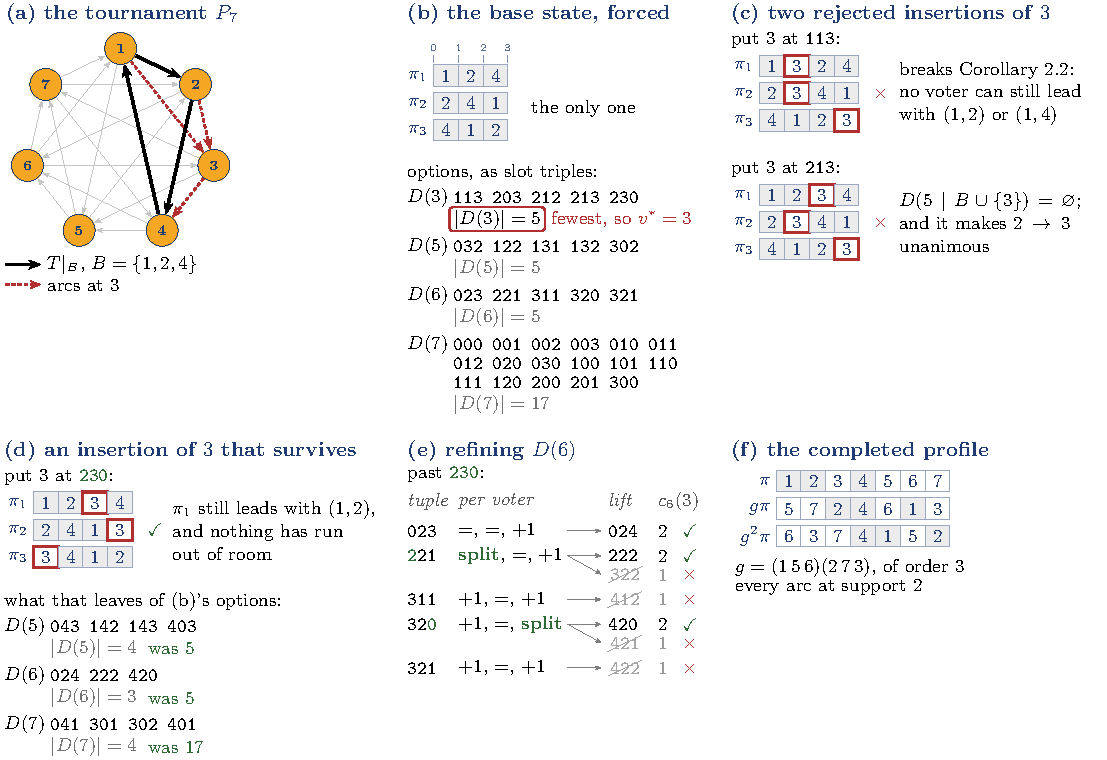
\includegraphics[width=\linewidth]{paley7_alg1.pdf}
\caption{Algorithm 1 on $P_7$ at $k = 3$, which is $3$-inducible, so the run ends in a witness. 
A \emph{slot triple} is one gap per voter, of the $4^{3} = 64$ available, and a vertex's domain is
those triples its arcs to $B$ admit. Here the base is $B = \mathrm{QR}$, the squares modulo 7, 
and Lemma 2.1 guarantees that at least one voter must rank 1 first and either 2 or 4 second. 
Ranking 4 second forces the other two voters to $241$, the only order getting both $4 \to 1$ and
$2 \to 4$ right, and $1 \to 2$ is then left with support $1$; so the base state in (b) is the only one.
\textbf{(a)} The base $T|_B$ on $B = \{1,2,4\}$ in bold; dashed, the arcs at the first vertex
inserted. \textbf{(b)} Steps 2--4: the base state is forced, and MRV takes the smallest domain.
\textbf{(c)} Two insertions the search rejects, one by Lemma 2.1 and one by leaving $5$ no slot at all.
\textbf{(d)} One that survives, and what it leaves of (b). \textbf{(e)} REFINE lifts each parent
tuple past the slot just used (unchanged below it, shifted above it, split where the two
coincide, which is what green marks), and the one new arc then keeps or kills each lift.
\textbf{(f)} The witness, every arc at support exactly $2$. Without Lemma 2.1 the search returns
all $7$ witnesses, a single orbit of $\mathrm{Aut}(P_7)$, of order $21$, so the profile is unique
up to symmetry, as Shepardson and Tovey (2009) report; $\pi$ generates the other two under the $g$
shown, the map $x \mapsto 2x + 4$ of $\mathbb{F}_7$.}
\end{figure}

\begin{center}\rule{0.5\linewidth}{0.5pt}\end{center}

\subsubsection{A.3 Integer programming and SAT are both too
slow}\label{a.3-integer-programming-and-sat-are-both-too-slow}

The natural integer program has one binary \(x_{v,ij}\) per voter \(v\)
and pair \(i < j\), meaning that \(v\) ranks \(i\) above \(j\), with
\(x_{v,ji}\) read as \(1 - x_{v,ij}\) so that antisymmetry is
structural. Each voter is forced to be a linear order by forbidding both
orientations of every \(3\)-cycle,
\[0 \;\le\; x_{v,ij} + x_{v,jl} - x_{v,il} \;\le\; 1 \qquad (i < j < l),\]
and the profile is forced to induce \(T\) by one majority row per arc,
\(\sum_{v} x_{v,ij} \ge (k+1)/2\). This is a pure feasibility problem.
At \(q = 23\), \(k = 5\) it has \(1{,}265\) binaries, \(17{,}710\)
transitivity rows and \(253\) majority rows.

The obstruction is structural rather than a deficiency of the solver.
Let us set \(x_{v,ij} = 3/5\) on every arc of \(T\) and \(2/5\) on every
non-arc, the same for all voters. Every cyclic triple then reads
\(3/5 + 3/5 - 2/5 = 4/5\) and every transitive one \(3/5\), both
interior to \([0,1]\), while every majority row is tight at exactly
\(3\). The relaxation is therefore feasible, and since the problem
carries no objective, LP feasibility yields no bound whatever:
branch-and-bound is left with nothing to prune by except infeasibility
discovered deep in the tree. That fractional point is also invariant
under both symmetry groups acting on the problem (the \(k!\) voter
relabellings and \(\mathrm{Aut}(T)\)), so it supplies no branching
direction either, and orbital branching recovers only the \(k!\) factor.
CPLEX and Gurobi both failed to close instances at \(n = 19\) within a
day.

The satisfiability encoding is \emph{dissent-Boolean}: one variable per
voter \(v\) and arc \(i \to j\) of \(T\), true when \(v\) ranks \(j\)
above \(i\) and so dissents from that arc. Each arc bounds its dissents,
at most \((k-1)/2\) of them for majority and exactly \((k-1)/2\) for
unit margin, and each voter's dissent set is forced to leave a linear
order triple by triple: a tournament is transitive exactly when it has
no directed \(3\)-cycle, so it is enough to forbid, for every voter and
every triple, the two dissent patterns that would make that triple
cyclic. For \(k = 5\) that is \(5\binom{n}{2}\) variables, \(15\)
clauses per arc at unit margin and \(10\) per triple. It is compact and
propagates well locally, and it is what both certified refutations of
Appendix B are built on.

Table 4 of Bachmeier et al.~(2019) reports their
\texttt{Sat-Check-k-Majority} on uniform random tournaments, tabulating
only entries whose average stays under 20 seconds. The \(k = 5\) column
reads

{\def\LTcaptype{none} % do not increment counter
\begin{longtable}[]{@{}llllllll@{}}
\toprule\noalign{}
\(n\) & 18 & 19 & 20 & 21 & 22 & 23 & 24 \\
\midrule\noalign{}
\endhead
\bottomrule\noalign{}
\endlastfoot
seconds & \(0.23\) & \(0.35\) & \(0.54\) & \(5.87\) & \(11.07\) &
\(18.95\) & --- \\
\end{longtable}
}

so on \emph{random} instances the method leaves the table between
\(n = 23\) and \(n = 24\), roughly doubling per added vertex. Random
tournaments are the easy case: no automorphisms to rediscover and, being
far from extremal, many witnesses. On the structured instance of the
same order, \(P_{23}\), the same solver did not terminate within a
cumulative six weeks. The gap between \(18.95\) seconds and six weeks at
equal \(n\) is the cost of symmetry.

A better encoding and an explicit symmetry break both help substantially
and are still not enough (results not shown). What does work is
supplying the solver with the decomposition itself: cube-and-conquer
over base states, which is how both refutations are certified in
Appendix B. A CDCL solver must otherwise discover that decomposition for
itself, and cannot exploit \(\mathrm{Aut}(T)\) at all without an
explicit break in the encoding.

\subsubsection{A.4 What makes the search
fast}\label{a.4-what-makes-the-search-fast}

Four choices make the search of Appendix A.2 fast, and the second is the
one that made \(n = 19\) and \(n = 23\) reasonable to compute.

\textbf{A dynamic variable order.} At every node we insert the unplaced
vertex minimising \(|D(v \mid S)|\), breaking ties toward the vertex
whose arcs to \(S\) are most imbalanced. The important part is that the
order is recomputed at every node rather than fixed per base state: on
Paley instances a static order is not competitive, because how
constrained a vertex is depends strongly on which part of the tournament
has already been placed.

\textbf{Incremental domain refinement.} Recomputing \(D(v \mid S)\) from
scratch at each node is the dominant cost of a naive implementation;
instead the child's domain is derived from the parent's by the three
cases in \texttt{REFINE} above, after which the single new arc filters
the lifted tuples by their support. Child domains are therefore
refinements of parent domains, computed in time proportional to the
surviving tuples rather than to the whole slot space, and domains live
in a stack-disciplined arena indexed by (depth, vertex) so that
backtracking is a pointer reset. Like for like this is worth a factor of
about \(110\) in wall time.

\textbf{Symmetry breaking.} The \(k!\) voter symmetry is absorbed
exactly by the base-state definition, which counts non-decreasing tuples
only. For \(\mathrm{Aut}(T)\) the engine imposes the anchoring of Lemma
2.1 or of Corollary 2.2, whichever is stronger on the tournament: the
condition is invariant under permuting voters, so it composes with the
base lex-order, and monotone under insertion, so it can be tested during
the search rather than only at the leaves.

\textbf{Early termination and caching by arc pattern.} A quick per-voter
agreement bound, obtained by counting the agreement between voter \(i\)
and the arcs between \(v\) and \(S\) two ways, proves \(D(v \mid S)\)
empty in \(O(k|S|)\) time without enumerating it. And the per-base-state
work is keyed by the \emph{arc pattern} of \(T|_B\) rather than by \(B\)
itself, so base-state counts, which depend only on that pattern, are
reused across every copy of the same base class and across every \(q\).

\textbf{Choosing the base.} The base set is not a free parameter, and
the fewest live base states is not the fastest choice: at \(q = 31\) the
class with \(4{,}007\) live states beat the class with \(2{,}537\),
whose states are individually slower, so we rank the twelve \(5\)-vertex
classes by the product of the live count and a sampled time per state
rather than by the count alone.

\subsubsection{\texorpdfstring{A.5 How the runtime scales in
\(q\)}{A.5 How the runtime scales in q}}\label{a.5-how-the-runtime-scales-in-q}

\textbf{A note on \(q = 27\).} The series below includes \(q = 27\), the
one prime power among the orders we computed with. Since \(27 = 3^3\),
\(P_{27}\) must be built over \(\mathbb{F}_{27}\) and not over
\(\mathbb{Z}/27\). \(P_{27}\) is the unique most symmetric doubly
regular tournament on \(27\) vertices, with
\(|\mathrm{Aut}(P_{27})| = 1053 = 3q(q-1)/2\), because the field
automorphisms contribute (in general \(|\mathrm{Aut}(P_q)| = q(q-1)e/2\)
when \(q = p^e\)). It is still transitive on arcs and on non-arcs, which
is what Lemma 2.1 needs. We ran \(q = 27\) to completion and it is not
\(5\)-inducible; since that does not bear on \(N(5)\) we report it here
only as a runtime datapoint.

On a fixed base decomposition the total runtime \emph{decreases} as the
tournament grows, and so does the node count: a larger Paley tournament
is \emph{more} constrained, so the search is refuted nearer the root and
the tree above each base state is smaller rather than larger. The work
per node moves the other way, rising monotonically from \(10.8\) to
\(57.4\) microseconds across the four runs below, because a larger
tournament carries larger domains and each refinement step costs more.
The node count falls faster than the per-node cost rises, which is what
makes the total fall. The full runs:

{\def\LTcaptype{none} % do not increment counter
\begin{longtable}[]{@{}
  >{\raggedright\arraybackslash}p{(\linewidth - 8\tabcolsep) * \real{0.0864}}
  >{\raggedright\arraybackslash}p{(\linewidth - 8\tabcolsep) * \real{0.2469}}
  >{\raggedright\arraybackslash}p{(\linewidth - 8\tabcolsep) * \real{0.1728}}
  >{\raggedright\arraybackslash}p{(\linewidth - 8\tabcolsep) * \real{0.1111}}
  >{\raggedright\arraybackslash}p{(\linewidth - 8\tabcolsep) * \real{0.3827}}@{}}
\toprule\noalign{}
\begin{minipage}[b]{\linewidth}\raggedright
\(q\)
\end{minipage} & \begin{minipage}[b]{\linewidth}\raggedright
live base states
\end{minipage} & \begin{minipage}[b]{\linewidth}\raggedright
core-hours
\end{minipage} & \begin{minipage}[b]{\linewidth}\raggedright
nodes
\end{minipage} & \begin{minipage}[b]{\linewidth}\raggedright
seconds per live base state
\end{minipage} \\
\midrule\noalign{}
\endhead
\bottomrule\noalign{}
\endlastfoot
23 & \(2{,}591\) & \(34.03\) & \(1.14 \times 10^{10}\) & \(47.3\) \\
27 & \(2{,}537\) & \(31.04\) & \(6.22 \times 10^{9}\) & \(44.0\) \\
31 & \(4{,}007\) & \(26.89\) & \(3.43 \times 10^{9}\) & \(24.2\) \\
43 & \(2{,}537\) & \(22.87\) & \(1.43 \times 10^{9}\) & \(32.5\) \\
\end{longtable}
}

\(P_{43}\) is decided in \emph{less time than \(P_{27}\)}, and explores
\(4.3\) times fewer nodes to do it. The last column is the third divided
by the second, so only the core-hours and the live base states are
measured. Just two of these four runs share a decomposition, \(q = 27\)
and \(q = 43\), on the same five-vertex base class and the same
\(2{,}537\) live base states; \(q = 23\) and \(q = 31\) each used their
own best configuration, and \(q = 31\)'s is the cheaper class of
Appendix A.2, which is why its per-state figure is the lowest of the
four. The core-hours fall monotonically in \(q\) either way. By
contrast, \(P_{43}\) minus a vertex takes \(185.5\) core-hours, far more
than \(P_{43}\) itself, as vertex deletion shrinks the automorphism
group.

Additionally, the search gets faster as the margin is tightened. On the
identical tournament (\(P_{43} -\,v\)), engine and \(5\)-vertex base
class, there is a factor of about \(90\). Requiring every arc to be at
unit margin admits \(2{,}200\) base states where majority admits
\(8{,}031\); additionally, under exact margin the last voter is
\emph{forced}, since the support accumulated over the first \(k-1\)
voters determines what the last must contribute, so a whole level of the
search collapses.

\textbf{Two machines, and why their runtimes are not comparable.} Some
computations ran on a cluster rather than the laptop. Measured across
six independent experiments, the cluster ran at \(2\) to \(5\) times the
laptop's runtime per unit of work.

We are not claiming that bespoke search beats ILP or SAT solvers in
general. Our engine is narrow: it exploits the specific facts that a
partial profile's extensions form a product of per-voter slot choices,
that this product refines monotonically, and that \(\mathrm{Aut}(T)\) is
large. For the specific Paley instances in this paper that the
general-purpose methods did not settle for us, the search settles in
hours on a single laptop.

\subsubsection{A.6 Runtimes for every
computation}\label{a.6-runtimes-for-every-computation}

All runs in this manuscript were performed on a single laptop (Apple
M-series, 14 cores, 24 GB RAM), using at most 11 cores concurrently,
with the following exceptions, which used a compute cluster: the census
of regular tournaments on \(15\) vertices, the self-converse census of
order \(13\), the order-\(12\) census of Appendix C, the two
\(22\)-vertex sweeps of Section 3.2, \(16\) of the \(19\) unrestricted
sweeps of doubly regular tournaments on \(23\) vertices in Section 3.7,
and most of the search of Appendix G. Runtimes are reported in
\emph{core-hours}, the workers' running times summed; cluster core-hours
are marked as such, and are not comparable with laptop ones (Appendix
A.5).

{\def\LTcaptype{none} % do not increment counter
\begin{longtable}[]{@{}
  >{\raggedright\arraybackslash}p{(\linewidth - 6\tabcolsep) * \real{0.5729}}
  >{\raggedright\arraybackslash}p{(\linewidth - 6\tabcolsep) * \real{0.1458}}
  >{\raggedright\arraybackslash}p{(\linewidth - 6\tabcolsep) * \real{0.1562}}
  >{\raggedleft\arraybackslash}p{(\linewidth - 6\tabcolsep) * \real{0.1250}}@{}}
\toprule\noalign{}
\begin{minipage}[b]{\linewidth}\raggedright
computation
\end{minipage} & \begin{minipage}[b]{\linewidth}\raggedright
margin
\end{minipage} & \begin{minipage}[b]{\linewidth}\raggedright
verdict
\end{minipage} & \begin{minipage}[b]{\linewidth}\raggedleft
core-hours
\end{minipage} \\
\midrule\noalign{}
\endhead
\bottomrule\noalign{}
\endlastfoot
\(P_{19}\), certified refutation & unit & not inducible & \(25.1\) \\
\(P_{23}\), certified refutation & unrestricted & not inducible &
\(236.0\) \\
\(\Delta_6 - 5\), certified refutation & unrestricted & not inducible &
\(1{,}292.7\) \\
\(\Delta_6 - 5\), sweep (cluster) & unrestricted & not inducible &
\(1{,}551.2\) \\
\(\Delta_{28} - 5\), sweep (cluster) & unrestricted & not inducible &
\(1{,}537.7\) \\
\(P_{31} -\,v\), sweep & unrestricted & not inducible & \(239.5\) \\
\(P_{23}\), one arc reversed & unrestricted & inducible & \(210.4\) \\
second doubly regular \(19\), all \(57\) arc reversals & unit & all
inducible & \(3.59\) \\
regular tournaments on \(15\) vertices (cluster) & unit & all inducible
& \(3{,}106\) \\
self-converse tournaments on \(13\) vertices (cluster) & unit & all
inducible & \(1{,}310\) \\
all tournaments on \(12\) vertices (cluster) & unit & all inducible &
\(\approx 10{,}000\) \\
\end{longtable}
}

The four full Paley sweeps, \(q = 23\), \(27\), \(31\) and \(43\), are
tabulated with their node counts in Appendix A.5.

\subsection{Appendix B. The formal
certificates}\label{appendix-b.-the-formal-certificates}

\subsubsection{B.1 The certified
refutations}\label{b.1-the-certified-refutations}

All three machine-checked results follow an established design rather
than a new one. \emph{Cube-and-conquer} is due to Heule, Kullmann,
Wieringa and Biere (2012): split a hard instance into many partial
assignments (\emph{cubes}), hand each to a CDCL solver, and let the
splitting supply the global structure the solver cannot find for itself.
The standard of \emph{proof} is the one Heule, Kullmann and Marek set
for the Boolean Pythagorean triples problem (Heule et al.~2016;
Cruz-Filipe et al.~2019), and Schur number five (Heule 2018) and the
Keller conjecture (Brakensiek et al.~2020) after it: every subproblem
emits a machine-checkable refutation, validated by an independent
checker rather than trusted. We claim no methodological novelty.

\textbf{What an LRAT proof is.} A solver's verdict of unsatisfiability
is not self-evidently checkable, so the solver writes a \emph{proof
log}: a file recording, in order, the clauses it derives, each of which
must follow from the input formula together with the clauses already
recorded, the last being the empty clause. A separate checker replays
that file and confirms every step, so what one trusts is the checker
rather than the solver. The available formats record essentially this
same derivation and differ mainly in how much work the replay costs. We
use LRAT (Cruz-Filipe et al.~2017), the format CaDiCaL emits natively
and \texttt{lrat-trim} consumes, in which checking is a single pass over
the file.

Two differences are consequences of our setting. Our cubes are
\emph{base states}, a combinatorial decomposition, which lets the
coverage of the cube set be certified separately (B.2) instead of
resting on a splitting heuristic. And where Heule et al.~(2016)
published a cube certificate from which its refutations can be
regenerated, we \emph{verify and discard}: each LRAT proof is checked,
hashed and deleted, and we only publish the hash value. The choice suits
the scale. Verifying the Boolean Pythagorean triples proof costs about
\(13{,}000\) core-hours to regenerate the refutations from the published
cube certificate (Heule 2016), and about \(16{,}000\) to check them
(Heule et al.~2016). Our certificates are orders of magnitude smaller:
\(25.1\) core-hours for \(P_{19}\), \(236.0\) for \(P_{23}\) and
\(1{,}292.7\) for \(\Delta_6 - 5\) cover solving \emph{and} checking.
Portable root values, which is exactly the check Section 5.2 supports,
can be easily compared by anyone replicating our computation.

For \(P_{19}\) at unit margin the instance is the dissent-Boolean
encoding of Appendix A.1 at \(q = 19\), \(k = 5\): \(855\) variables and
\(12{,}255\) clauses. The cubes are the \(142{,}251\) base states of the
\(6\)-vertex base \(\{1,2,3,4,5,12\}\), of which \(22{,}876\) survive
the arc-orbit break, and each is handed whole to CaDiCaL with
\texttt{-\/-lrat=true\ -\/-checkproof=0}. Each LRAT proof is checked by
\texttt{lrat-trim}. The runtime was \(2.64\) hours on ten cores. Its
coverage half is the same construction as the one below, at
\(143{,}032\) clauses, and solves in \(7.56\) seconds.

For the \(P_{23}\) refutation of Section 3.1, the base is
\(\{1,2,3,4,6,7\}\) with \(3{,}414{,}729\) base states, of which
\(343{,}896\) survive the arc-orbit and non-arc-orbit breaks; every one
is unsatisfiable, with an LRAT proof independently verified by
\texttt{lrat-trim}. The runtime was \(21.72\) hours on eleven cores. The
coverage half of the proof is a single unsatisfiable instance of \(350\)
constraint clauses, \(356\) symmetry-breaking clauses and
\(3{,}414{,}729\) negated cubes, one per base state, since coverage must
see \emph{every} base state whereas the orbit breaks apply to the search
half only. It solves in just under \(20\) minutes on one core and emits
a \(2.05\) GiB LRAT proof.

For the \(\Delta_6 - 5\) refutation of Section 3.2 the instance is the
dissent-Boolean encoding at \(n = 22\) and plain majority: \(1{,}155\)
variables and \(17{,}710\) clauses. The tournament has no non-trivial
automorphism, so there is no orbit break, and all \(742{,}374\) base
states of the six-vertex base \(\{1,2,3,4,13,19\}\) (in the labelling of
\(\Delta_6\)) are cubes; every one is unsatisfiable, with an LRAT proof
independently verified by \texttt{lrat-trim}. The runtime was about
\(118\) hours on eleven cores. The coverage half is the same
construction as for \(P_{23}\), with \(742{,}374\) negated cubes, and
solves in \(82.8\) seconds on one core. This refutation is the most
expensive of the three, although its tournament is the smallest: with no
automorphisms there is nothing to break, so every base state reaches the
solver, against one in ten for \(P_{23}\).

\subsubsection{B.2 What the certificates do and do not
establish}\label{b.2-what-the-certificates-do-and-do-not-establish}

The trust chain has four links:

{\def\LTcaptype{none} % do not increment counter
\begin{longtable}[]{@{}
  >{\raggedright\arraybackslash}p{(\linewidth - 2\tabcolsep) * \real{0.5000}}
  >{\raggedright\arraybackslash}p{(\linewidth - 2\tabcolsep) * \real{0.5000}}@{}}
\toprule\noalign{}
\begin{minipage}[b]{\linewidth}\raggedright
link
\end{minipage} & \begin{minipage}[b]{\linewidth}\raggedright
status
\end{minipage} \\
\midrule\noalign{}
\endhead
\bottomrule\noalign{}
\endlastfoot
every live cube is unsatisfiable & machine-checked: CaDiCaL, rechecked
by \texttt{lrat-trim} \\
the cubes cover every lex-canonical base assignment & machine-checked:
LRAT, verified by \texttt{lrat-trim} \\
(L1) orbit anchoring loses no generality & human-checked: Lemma 2.1 \\
(L2) lex-ordering the voters loses no generality & human-checked: Lemma
2.3 \\
\end{longtable}
}

The two human-checked links are proved in Section 2. Lemma 2.1 is what
licenses solving only the \emph{live} cubes, in its arc/non-arc form:
\(\mathrm{Aut}(P_q)\) is transitive on arcs and on non-arcs, so a
voter's top pair may be assumed to be a fixed arc or a fixed non-arc.
Lemma 2.3 licenses the lex chain in the coverage computation. For
\(\Delta_6 - 5\) the chain is one link shorter: with no automorphism to
exploit, no orbit break is applied and Lemma 2.1 is not used, so only
Lemma 2.3 remains human-checked. The lemmas are human-checked links not
because they are doubtful but because nothing in the pipeline checks
them; the depth-first engine inherits them, but shares no implementation
with this one, so their agreement is evidence about the implementations,
not the lemmas.

\subsection{Appendix C. The order-12 case
analysis}\label{appendix-c.-the-order-12-case-analysis}

Every tournament on \(12\) vertices is \(5\)-inducible, so
\(N(5) \ge 13\). This appendix describes that computation. It is one of
the results in this paper that was not run on the laptop of Section 3:
it ran on a shared cluster, and its runtime is reported in cluster
core-hours (see Appendix A.5).

\subsubsection{C.1 Reduction to one-vertex
extensions}\label{c.1-reduction-to-one-vertex-extensions}

A direct census is out of reach: \(D_{12} \approx 1.5 \times 10^{11}\)
classes, \(170\) times the order-\(11\) census of Chindelevitch and
Harutyunyan (2026). We use that census as the outer loop instead. Let us
write \(L + S\) for the tournament obtained from an order-\(11\)
tournament \(L\) by adding a vertex \(v\) whose out-neighbourhood is
\(S \subseteq V(L)\). Two observations simplify the analysis.

\textbf{(C1)} Every order-\(12\) tournament is \(L + S\) for some
order-\(11\) \(L\) and some \(S\).

\textbf{(C2)} Restricting a profile that realises \(L + S\) to \(V(L)\)
gives a profile that realises \(L\).

By (C1), enumerating all \(D_{11}\) order-\(11\) classes and settling
all \(2^{11} = 2{,}048\) extensions of each settles every order-\(12\)
tournament; all of the former are \(5\)-inducible by the census of
Chindelevitch and Harutyunyan (2026), which is what makes the outer loop
available. By (C2), a profile realising \(L + S\) may be sought by
\emph{inserting} \(v\) into a profile realising \(L\) with no loss of
generality, since every profile for \(L+S\) arises that way. That is
what phase 1 exploits.

\subsubsection{C.2 Three phases}\label{c.2-three-phases}

The census is organised into three phases, with the fastest ones
occurring earlier.

\textbf{Phase 1, the covering search.} Rather than \(2{,}048\) separate
instances per order-\(11\) tournament, one search enumerates profiles
realising \(L\) \emph{at unit margin} and, for each, records every
out-neighbourhood obtainable by inserting \(v\) into its five orders:
\(v\)'s position in each order is a threshold, and the support of
\(v \to u\) is the number of orders that place \(v\) above \(u\), so one
traversal certifies many extensions at once. This is the engine of
Appendix A.2 with \(v\)'s placement read off rather than fixed in
advance. The margin makes this phase pay twice: it keeps the enumeration
of profiles for \(L\) small, and a unit-margin witness is in particular
a majority witness, so every extension the phase covers is settled in
both regimes at once. The phase is one-sided: an extension it covers is
certified \(5\)-inducible, but one left over is not refuted. This phase
settles every one of the \(2{,}048\) extensions of \(99.5\%\) of the
order-\(11\) tournaments.

\textbf{Phase 2, deciding what is left.} Each extension phase 1 leaves
open is materialised as an order-\(12\) tournament \(L + S\) and decided
by the same engine, again at unit margin, where a witness settles it
positively. About one extension in \(200{,}000\) reached this phase, and
every one of them is \(5\)-inducible with unit margin.

\textbf{Phase 3, plain majority.} Only a \emph{majority} refutation
would be a counterexample, so any instance negative at unit margin is
re-run without the margin restriction. Phase 3 was never invoked: every
tournament was settled at unit margin, so the weaker question never had
to be asked.

\subsubsection{C.3 One tournament of each converse
pair}\label{c.3-one-tournament-of-each-converse-pair}

If \(\pi_1, \dots, \pi_5\) realise \(T\), their reversals realise the
converse \(\bar{T}\), with the same margins, so \(T\) is \(5\)-inducible
if and only if \(\bar{T}\) is. Moreover
\(\overline{L + S} = \bar{L} + (V(L) \setminus S)\), so settling all
\(2{,}048\) extensions of \(L\) settles all \(2{,}048\) of \(\bar{L}\)
as well. We therefore keep one tournament of each converse pair, by the
rule that \(L\) is kept if and only if
\(\mathrm{canon}(L) \le \mathrm{canon}(\bar{L})\). This keeps exactly
one of each pair together with every self-converse tournament,
\((D_{11} + S_{11})/2\) in all, where \(S_{11}\) is the number of
self-converse order-\(11\) classes; this saves a factor of
\(\lessapprox 2\). We also check the number of tournaments kept is
\((D_{11} + S_{11})/2\).

Total runtime: approximately \(10{,}000\) cluster core-hours. The search
code, the per-part records and the roll-up are at
\texttt{cluster/jz\_n12cover} in the repository of Section 5.

\subsection{Appendix D. Exact enumeration
counts}\label{appendix-d.-exact-enumeration-counts}

In this table, \(D_n\), \(R_n\) and \(S_n\) are the numbers of
isomorphism classes of all, of regular, and of self-converse tournaments
on \(n\) vertices. They match OEIS A000568 (OEIS Foundation Inc.~2026a),
A096368 (OEIS Foundation Inc.~2026c), and A002785 (OEIS Foundation
Inc.~2026b).

{\def\LTcaptype{none} % do not increment counter
\begin{longtable}[]{@{}rrrr@{}}
\toprule\noalign{}
\(n\) & \(D_n\) & \(R_n\) & \(S_n\) \\
\midrule\noalign{}
\endhead
\bottomrule\noalign{}
\endlastfoot
\(11\) & \(903{,}753{,}248\) & \(1{,}223\) & \(279{,}968\) \\
\(12\) & \(154{,}108{,}311{,}168\) & --- & \(1{,}492{,}288\) \\
\(13\) & --- & \(1{,}495{,}297\) & \(95{,}458{,}560\) \\
\(15\) & --- & \(18{,}400{,}989{,}629\) & --- \\
\end{longtable}
}

\subsection{\texorpdfstring{Appendix E. Locally transitive tournaments,
at unit margin, for every odd
\(k \geq 3\)}{Appendix E. Locally transitive tournaments, at unit margin, for every odd k \textbackslash geq 3}}\label{appendix-e.-locally-transitive-tournaments-at-unit-margin-for-every-odd-k-geq-3}

\setcounter{figure}{0}\renewcommand{\thefigure}{E.\arabic{figure}}

A tournament is \emph{locally transitive} if for every vertex \(v\) both
\(N^{+}(v)\) and \(N^{-}(v)\) induce transitive subtournaments.
Equivalently it is \emph{round}: the vertices admit a cyclic order
\(v_0, \dots, v_{n-1}\) in which every \(N^{-}(v) \cup \{v\}\) and
\(\{v\} \cup N^{+}(v)\) is an interval, so that, orienting the cyclic
order along the arcs, each vertex beats exactly the
\(d_i = |N^{+}(v_i)|\) vertices that follow it:
\(N^{+}(v_i) = \{v_{i+1}, \dots, v_{i+d_i}\}\), indices modulo \(n\).
The equivalence is due to Brouwer (1980), who proved it in the course of
enumerating the class, and to Alspach and Tabib (1982), who state it for
tournaments under the name \emph{domination orientable}; Bang-Jensen
later generalised it to digraphs.

\textbf{Theorem E.1.} \emph{Every locally transitive tournament is
\(3\)-inducible with unit margin, and hence \(k\)-inducible with unit
margin for every odd \(k \ge 3\).}

\begin{figure}[!htbp]
\centering
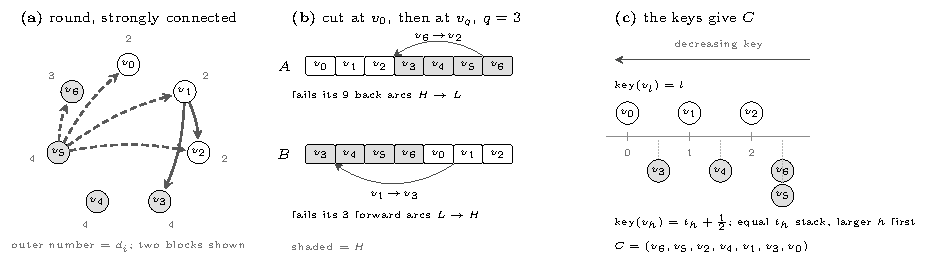
\includegraphics[width=\linewidth]{roundE.pdf}
\caption{The construction of Appendix E on a round tournament with out-degree sequence
$(2, 2, 2, 4, 4, 4, 3)$, for which $q = 3$. \textbf{(a)} The cyclic order, each $v_i$ labelled with its
out-degree $d_i$, so that its out-neighbours are $v_{i+1}, \dots, v_{i+d_i}$; the two blocks drawn
are those of $v_1 \in L$ and $v_5 \in H$, and that of $v_5$ wraps, with back-targets $v_0, v_1, v_2$.
\textbf{(b)} $A$ and $B$ are the same cyclic order cut at $v_0$ and at $v_q$, each failing exactly the
arcs that cross its own cut, $9$ back arcs and $3$ forward arcs; one of each is drawn.
\textbf{(c)} The keys, $C$ being the vertices in decreasing order of key.
A vertex of $L$ sits at its index and one of $H$ half a unit past its ceiling, so
reading leftwards puts $v_h$ before $v_l$ exactly when $v_h \to v_l$; $v_5$ and $v_6$ share a
ceiling and the tie-break separates them, giving $C = (v_6, v_5, v_2, v_4, v_1, v_3, v_0)$.}
\end{figure}

A locally transitive tournament that is not strongly connected is
transitive: a strongly connected component \(C\) with \(|C| \geq 3\)
contains a directed triangle, and any vertex outside \(C\) either beats
all of \(C\) or loses to all of it, contradicting local transitivity. A
transitive tournament is \(1\)-inducible at margin \(1\), its single
voter supporting every arc. Adding an order together with its reverse
adds one supporter and one opponent to each arc, raising every support
by \(1\) and \(k\) by \(2\) and so leaving every margin \(2c(e) - k\)
unchanged. Padding with the identity order \((1, 2, \dots, n)\) and its
reverse therefore gives unit margin at \(k = 3\), and repeating gives
every odd \(k\).

Let \(T\) be strongly connected and round, and let \(d_i\) be the
out-degree of vertex \(i\); Figure E.1 illustrates what follows, on
seven vertices. Cutting the cyclic order at \(v_0\) gives the linear
order \(A = (v_0, \dots, v_{n-1})\). We write \(r_i = i + d_i\), an
integer deliberately \emph{not} reduced modulo \(n\). For each \(v_i\),
the out-neighbours are then \(v_{i+1}, \dots, v_{r_i}\) with indices
reduced only when they are read as vertices. The sequence \(r\) is
non-decreasing, since if \(r_{i+1} < r_i\) then \(v_{r_{i+1}+1}\) is an
out-neighbour of \(v_i\), while its own interval includes \(v_i\), a
contradiction. Let \(H = \{i : r_i \ge n\}\) be the vertices with an
out-neighbour that the cut defined by \(A\) placed \emph{before} them.
As \(r\) is non-decreasing, \(H = \{q, \dots, n-1\}\) for some \(q\);
write \(L = \{0, \dots, q-1\}\). Neither set is empty: \(H = \emptyset\)
would make \(v_{n-1}\) a sink and \(L = \emptyset\) would force
\(d_0 \ge n\), so neither occurs. For \(h \in H\) put \(t_h = r_h - n\),
so that the out-neighbours of \(v_h\) placed before it by the cut are
exactly \(v_0, \dots, v_{t_h}\): we call them the \emph{back-targets} of
\(v_h\), and \(t_h\) its \emph{ceiling}. By monotonicity of \(r\),
\(t_q \le \dots \le t_{n-1}\). Every back-target lies in \(L\), that is
\(t_{n-1} < q\): otherwise \(v_{n-1} \to v_q\), while \(r_q \ge n\)
implies \(v_q \to v_{n-1}\). The arcs between \(L\) and \(H\) therefore
divide into the \emph{back arcs} going from \(H\) to \(L\), and the
\emph{forward arcs} going from \(L\) to \(H\); and for \(h \in H\) and
\(l \in L\) we have \(v_h \to v_l\) exactly when \(l \le t_h\).

We give each vertex a \emph{key}: \(\mathrm{key}(v_l) = l\) for
\(l \in L\) and \(\mathrm{key}(v_h) = t_h + \tfrac12\) for \(h \in H\),
ties among equal ceilings broken in favour of the larger index, and let
\(C\) list the vertices in decreasing order of key. Integer and
half-integer keys never collide, so that tie-break is the only one
needed, the keys are pairwise distinct and \(C\) is a linear order; and
for \(h \in H\) and \(l \in L\),
\(\mathrm{key}(v_h) > \mathrm{key}(v_l) \iff t_h + \tfrac12 > l \iff l \le t_h \iff v_h \to v_l\),
so \(C\) places \(v_h\) before \(v_l\) exactly when \(v_h \to v_l\). We
now take the three orders \(A = (v_0, \dots, v_{n-1})\),
\(B = (v_q, \dots, v_{n-1}, v_0, \dots, v_{q-1})\), which is the same
cyclic order cut at \(v_q\) instead of at \(v_0\), and \(C\). Every arc
is now easily seen to have support exactly two. \emph{Arcs with both
endpoints inside \(L\) or inside \(H\)} are only supported by \(A\) and
\(B\); \emph{forward arcs \(v_l \to v_h\)} are only supported by \(A\)
and \(C\); and \emph{back arcs \(v_h \to v_l\)} are only supported by
\(B\) and \(C\), so the profile realises \(T\) at unit margin. The
padding argument above extends this margin to any odd \(k \geq 3\).
\(\blacksquare\)

\subsection{\texorpdfstring{Appendix F. Criticality at \(21\)
vertices}{Appendix F. Criticality at 21 vertices}}\label{appendix-f.-criticality-at-21-vertices}

This appendix carries the detail behind Section 3.6. Throughout, \(h\)
ranges over the four unit-margin obstructions among the \(110\)
vertex-transitive tournaments on \(21\) vertices (Section 3.7).

\textbf{Vertex-critical but maximally not arc-critical.} Arc-criticality
implies vertex-criticality, and the converse fails here as widely as it
can. Each \(h\) is \emph{vertex-critical} at unit margin, and for
\(h_1\) every single-arc reversal remains a unit-margin obstruction.

\textbf{Arc-criticality is a property of the arc, not just the
tournament.} All four have ten arc orbits of size \(21\); we sweep one
representative per orbit at unit margin and get results that differ by
tournament \emph{and} by arc, \texttt{U} marking a reversal that is
still not unit-margin inducible and \texttt{S} one that is. \(h_2\)
splits five orbits to five, so exactly half its arcs are critical and we
call it \emph{arc-semi-critical}; with \(P_{23}\) arc-critical
unrestricted and \(h_1\) critical nowhere, all three possibilities occur
among our tournaments. Intriguingly, every one of the \(15\) reversals
that remains an obstruction belongs to a tournament with \emph{cyclic
automorphism group}, while all \(20\) orbits of the two with the
nonabelian group of order \(21\) are inducible.

{\def\LTcaptype{none} % do not increment counter
\begin{longtable}[]{@{}
  >{\raggedright\arraybackslash}p{(\linewidth - 6\tabcolsep) * \real{0.2500}}
  >{\raggedright\arraybackslash}p{(\linewidth - 6\tabcolsep) * \real{0.2500}}
  >{\raggedright\arraybackslash}p{(\linewidth - 6\tabcolsep) * \real{0.2500}}
  >{\raggedright\arraybackslash}p{(\linewidth - 6\tabcolsep) * \real{0.2500}}@{}}
\toprule\noalign{}
\begin{minipage}[b]{\linewidth}\raggedright
tournament
\end{minipage} & \begin{minipage}[b]{\linewidth}\raggedright
\(\mathrm{Aut}\)
\end{minipage} & \begin{minipage}[b]{\linewidth}\raggedright
the ten orbits
\end{minipage} & \begin{minipage}[b]{\linewidth}\raggedright
obstructions
\end{minipage} \\
\midrule\noalign{}
\endhead
\bottomrule\noalign{}
\endlastfoot
\(h_1\) & \(\mathbb{Z}_{21}\) & \texttt{U\ U\ U\ U\ U\ U\ U\ U\ U\ U} &
\(10\) \\
\(h_2\) & \(\mathbb{Z}_{21}\) & \texttt{U\ S\ U\ S\ S\ U\ U\ S\ S\ U} &
\(5\) \\
\(h_4\), \(h_5\) & \(\mathbb{Z}_7 \rtimes \mathbb{Z}_3\) &
\texttt{S\ S\ S\ S\ S\ S\ S\ S\ S\ S} & \(0\) \\
\end{longtable}
}

\subsection{Appendix G. The search below 22
vertices}\label{appendix-g.-the-search-below-22-vertices}

This appendix summarises the search for an obstruction on fewer than
\(22\) vertices, which would improve the upper bound of Section 3.2. It
has found none.

The search runs downward, because \(5\)-inducibility is inherited by
subtournaments: restricting a witness for \(T\) to a subset of the
vertices gives a witness for the subtournament. An obstruction on fewer
vertices therefore lies below some larger one, and the natural place to
look is among the vertex deletions of known obstructions. A host is
settled positively as soon as one base state yields a witness, which is
cheap, and negatively only by a complete search, which is not; so each
level is first screened for witnesses, and only hosts that resist the
screen are searched further.

The starting points are the \(36\) doubly regular tournaments on \(23\)
vertices other than \(P_{23}\), all of which are obstructions (Section
3.7). \(P_{23}\) itself is excluded, since \(P_{23} - v\) is
\(5\)-inducible (Section 3.6) and so, by inheritance, is every
tournament below it. Up to isomorphism and up to taking the converse,
the levels below the \(36\) are as follows.

{\def\LTcaptype{none} % do not increment counter
\begin{longtable}[]{@{}
  >{\raggedleft\arraybackslash}p{(\linewidth - 6\tabcolsep) * \real{0.0533}}
  >{\raggedleft\arraybackslash}p{(\linewidth - 6\tabcolsep) * \real{0.0533}}
  >{\raggedleft\arraybackslash}p{(\linewidth - 6\tabcolsep) * \real{0.0533}}
  >{\raggedright\arraybackslash}p{(\linewidth - 6\tabcolsep) * \real{0.8400}}@{}}
\toprule\noalign{}
\begin{minipage}[b]{\linewidth}\raggedleft
vertices
\end{minipage} & \begin{minipage}[b]{\linewidth}\raggedleft
deleted
\end{minipage} & \begin{minipage}[b]{\linewidth}\raggedleft
classes
\end{minipage} & \begin{minipage}[b]{\linewidth}\raggedright
status
\end{minipage} \\
\midrule\noalign{}
\endhead
\bottomrule\noalign{}
\endlastfoot
\(22\) & \(1\) & \(378\) & \(2\) searched completely, both obstructions
(Section 3.2) \\
\(21\) & \(2\) & \(4{,}108\) & \(1{,}173\) settled, all
\(5\)-inducible \\
\(20\) & \(3\) & \(28{,}724\) & all \(5\)-inducible \\
\end{longtable}
}

At \(22\) vertices all \(378\) classes were first screened at up to
\(50\) base states each, without a single witness, and the two complete
searches were chosen from among them. At \(21\) vertices the \(1{,}173\)
settled classes include all \(506\) two-vertex deletions of \(\Delta_6\)
and \(\Delta_{28}\), so every \(21\)-vertex subtournament of either
parent is \(5\)-inducible, and in particular both \(22\)-vertex
obstructions are vertex-critical. The other settled classes are a
stratified random sample of \(400\), all \(53\) classes below
\(\Delta_{11}\), and every class obtained by deleting vertex \(5\)
together with one other vertex, the deletion that produced both
obstructions; the remaining \(2{,}935\) classes are open. At \(20\)
vertices every class is \(5\)-inducible, and so, by inheritance, is
every tournament on \(19\) vertices or fewer below the \(36\).

Witnesses become rarer as one climbs. At \(21\) vertices about one base
state in \(110\) yields a witness; at \(22\) vertices the screen
exhausted \(13{,}863\) base states and found none. A host at \(21\)
vertices therefore costs a few dozen cluster core-hours to settle, and
an obstruction at \(22\) about \(1{,}500\) to prove.

Two obstructions on \(25\) vertices from other families were descended
the same way: \(P_{27}\) with two vertices deleted, and the circulant
tournament on \(25\) vertices in which every arc lies in six directed
triangles. Neither is \(5\)-inducible, by complete searches, and every
\(21\)-vertex subtournament of either is \(5\)-inducible, so neither
family yields an obstruction below \(22\).

\end{document}
